%  LaTeX support: latex@mdpi.com 
%  For support, please attach all files needed for compiling as well as the log file, and specify your operating system, LaTeX version, and LaTeX editor.

%=================================================================
\documentclass[sensors,article,submit,moreauthors,pdftex]{Definitions/mdpi} 

% For posting an early version of this manuscript as a preprint, you may use "preprints" as the journal and change "submit" to "accept". The document class line would be, e.g., \documentclass[preprints,article,accept,moreauthors,pdftex]{mdpi}. This is especially recommended for submission to arXiv, where line numbers should be removed before posting. For preprints.org, the editorial staff will make this change immediately prior to posting.

%--------------------
% Class Options:
%--------------------
%----------
% journal
%----------
% Choose between the following MDPI journals:
% acoustics, actuators, addictions, admsci, adolescents, aerospace, agriculture, agriengineering, agronomy, ai, algorithms, allergies, analytica, animals, antibiotics, antibodies, antioxidants, appliedchem, applmech, applmicrobiol, applnano, applsci, arts, asi, atmosphere, atoms, audiolres, automation, axioms, batteries, bdcc, behavsci, beverages, biochem, bioengineering, biologics, biology, biomechanics, biomedicines, biomedinformatics, biomimetics, biomolecules, biophysica, biosensors, biotech, birds, bloods, brainsci, buildings, businesses, cancers, carbon, cardiogenetics, catalysts, cells, ceramics, challenges, chemengineering, chemistry, chemosensors, chemproc, children, civileng, cleantechnol, climate, clinpract, clockssleep, cmd, coatings, colloids, compounds, computation, computers, condensedmatter, conservation, constrmater, cosmetics, crops, cryptography, crystals, curroncol, cyber, dairy, data, dentistry, dermato, dermatopathology, designs, diabetology, diagnostics, digital, disabilities, diseases, diversity, dna, drones, dynamics, earth, ebj, ecologies, econometrics, economies, education, ejihpe, electricity, electrochem, electronicmat, electronics, encyclopedia, endocrines, energies, eng, engproc, entropy, environments, environsciproc, epidemiologia, epigenomes, fermentation, fibers, fire, fishes, fluids, foods, forecasting, forensicsci, forests, fractalfract, fuels, futureinternet, futuretransp, futurepharmacol, futurephys, galaxies, games, gases, gastroent, gastrointestdisord, gels, genealogy, genes, geographies, geohazards, geomatics, geosciences, geotechnics, geriatrics, hazardousmatters, healthcare, hearts, hemato, heritage, highthroughput, histories, horticulturae, humanities, hydrogen, hydrology, hygiene, idr, ijerph, ijfs, ijgi, ijms, ijns, ijtm, ijtpp, immuno, informatics, information, infrastructures, inorganics, insects, instruments, inventions, iot, j, jcdd, jcm, jcp, jcs, jdb, jfb, jfmk, jimaging, jintelligence, jlpea, jmmp, jmp, jmse, jne, jnt, jof, joitmc, jor, journalmedia, jox, jpm, jrfm, jsan, jtaer, jzbg, kidney, land, languages, laws, life, liquids, literature, livers, logistics, lubricants, machines, macromol, magnetism, magnetochemistry, make, marinedrugs, materials, materproc, mathematics, mca, measurements, medicina, medicines, medsci, membranes, metabolites, metals, metrology, micro, microarrays, microbiolres, micromachines, microorganisms, minerals, mining, modelling, molbank, molecules, mps, mti, nanoenergyadv, nanomanufacturing, nanomaterials, ncrna, network, neuroglia, neurolint, neurosci, nitrogen, notspecified, nri, nursrep, nutrients, obesities, oceans, ohbm, onco, oncopathology, optics, oral, organics, osteology, oxygen, parasites, parasitologia, particles, pathogens, pathophysiology, pediatrrep, pharmaceuticals, pharmaceutics, pharmacy, philosophies, photochem, photonics, physchem, physics, physiolsci, plants, plasma, pollutants, polymers, polysaccharides, proceedings, processes, prosthesis, proteomes, psych, psychiatryint, publications, quantumrep, quaternary, qubs, radiation, reactions, recycling, regeneration, religions, remotesensing, reports, reprodmed, resources, risks, robotics, safety, sci, scipharm, sensors, separations, sexes, signals, sinusitis, smartcities, sna, societies, socsci, soilsystems, solids, sports, standards, stats, stresses, surfaces, surgeries, suschem, sustainability, symmetry, systems, taxonomy, technologies, telecom, textiles, thermo, tourismhosp, toxics, toxins, transplantology, traumas, tropicalmed, universe, urbansci, uro, vaccines, vehicles, vetsci, vibration, viruses, vision, water, wevj, women, world 

%---------
% article
%---------
% The default type of manuscript is "article", but can be replaced by: 
% abstract, addendum, article, book, bookreview, briefreport, casereport, comment, commentary, communication, conferenceproceedings, correction, conferencereport, entry, expressionofconcern, extendedabstract, datadescriptor, editorial, essay, erratum, hypothesis, interestingimage, obituary, opinion, projectreport, reply, retraction, review, perspective, protocol, shortnote, studyprotocol, systematicreview, supfile, technicalnote, viewpoint, guidelines, registeredreport, tutorial
% supfile = supplementary materials

%----------
% submit
%----------
% The class option "submit" will be changed to "accept" by the Editorial Office when the paper is accepted. This will only make changes to the frontpage (e.g., the logo of the journal will get visible), the headings, and the copyright information. Also, line numbering will be removed. Journal info and pagination for accepted papers will also be assigned by the Editorial Office.

%------------------
% moreauthors
%------------------
% If there is only one author the class option oneauthor should be used. Otherwise use the class option moreauthors.

%---------
% pdftex
%---------
% The option pdftex is for use with pdfLaTeX. If eps figures are used, remove the option pdftex and use LaTeX and dvi2pdf.

%=================================================================
% MDPI internal commands
\firstpage{1} 
\makeatletter 
\setcounter{page}{\@firstpage} 
\makeatother
\pubvolume{1}
\issuenum{1}
\articlenumber{0}
\pubyear{2021}
\copyrightyear{2020}
%\externaleditor{Academic Editor: Firstname Lastname} % For journal Automation, please change Academic Editor to "Communicated by"
\datereceived{} 
\dateaccepted{} 
\datepublished{} 
\hreflink{https://doi.org/} % If needed use \linebreak
%------------------------------------------------------------------
% The following line should be uncommented if the LaTeX file is uploaded to arXiv.org
%\pdfoutput=1

%=================================================================
% Add packages and commands here. The following packages are loaded in our class file: fontenc, inputenc, calc, indentfirst, fancyhdr, graphicx, epstopdf, lastpage, ifthen, lineno, float, amsmath, setspace, enumitem, mathpazo, booktabs, titlesec, etoolbox, tabto, xcolor, soul, multirow, microtype, tikz, totcount, changepage, paracol, attrib, upgreek, cleveref, amsthm, hyphenat, natbib, hyperref, footmisc, url, geometry, newfloat, caption

%=================================================================
%% Please use the following mathematics environments: Theorem, Lemma, Corollary, Proposition, Characterization, Property, Problem, Example, ExamplesandDefinitions, Hypothesis, Remark, Definition, Notation, Assumption
%% For proofs, please use the proof environment (the amsthm package is loaded by the MDPI class).

%=================================================================
% Full title of the paper (Capitalized)
\Title{Fast Obstacle Detection and Recognition for Unmanned Surface Vehicles}

% MDPI internal command: Title for citation in the left column
\TitleCitation{Fast Obstacle Detection and Recognition for Unmanned Surface Vehicles}

% Author Orchid ID: enter ID or remove command
\newcommand{\orcidauthorA}{0000-0001-7596-3598} % Add \orcidA{} behind the author's name
%\newcommand{\orcidauthorB}{0000-0000-0000-000X} % Add \orcidB{} behind the author's name

% Authors, for the paper (add full first names)
\Author{Shanliang Yao $^{1}$\orcidA{}, Xiaohui Zhu $^{1}$ *, Yong Yue $^{1}$, Yutao Yue $^{2}$, Tianlei Shi $^{1}$, Kaiyuan Yang $^{1}$ and Yijie Chu $^{1}$}

% MDPI internal command: Authors, for metadata in PDF
\AuthorNames{Shanliang Yao, Xiaohui Zhu, Yong Yue, Yutao Yue, Tianlei Shi, Kaiyuan Yang, Yijie Chu.}

% MDPI internal command: Authors, for citation in the left column
\AuthorCitation{Yao, S; Zhu, X; Yue, Y; Yue, Y; Shi, T; Yang, K; Chu, Y.}
% If this is a Chicago style journal: Lastname, Firstname, Firstname Lastname, and Firstname Lastname.

% Affiliations / Addresses (Add [1] after \address if there is only one affiliation.)
\address{%
$^{1}$ \quad Department of Computer Science and Software Engineering, Xi’an Jiaotong-Liverpool University, Suzhou 215123, China; Shanliang.Yao19@student.xjtlu.edu.cn\\
 $^{2}$ \quad DPI; e-mail@e-mail.com
}

% Contact information of the corresponding author
\corres{Correspondence: Xiaohui.Zhu@xjtlu.edu.cn;}

% Current address and/or shared authorship
%\firstnote{Current address: Affiliation 3} 
%\secondnote{These authors contributed equally to this work.}
% The commands \thirdnote{} till \eighthnote{} are available for further notes

%\simplesumm{} % Simple summary

%\conference{} % An extended version of a conference paper

% Abstract (Do not insert blank lines, i.e. \\) 
\abstract{Unmanned Surface Vehicles (USVs) play an essential role in water quality monitoring, riverbed mapping, river rescue, and underwater detection. One of the significant challenges for USVs is obstacle detection and recognition of all kinds of objects such as boats, buoys and garbage floating on the water surface. 
This research aims to construct an obstacle detection model with high accuracy and high speed. Thus, we create a new river surface obstacle dataset from the video data captured by the USV during its sailing. Besides, the pre-trained weight trained on the Common Objects in Context (COCO) dataset is adopted to implement the training of the PaddlePaddle - You Only Look Once (PP-YOLO) model based on the PP-YOLO algorithm.
Moreover, a vision-based obstacle detection method for USVs is proposed to detect and recognize the locations and categories of the obstacles from the live video stream captured by the camera on the USV.
We also propose a novel PP-YOLO-mobile model based on the PP-YOLO model by replacing the backbone with MobileNetV2 and adding a data augmentation method. The experimental results show that compared with the original PP-YOLO model, the mean average precision (mAP) under the PP-YOLO-mobile model is improved by 2.7392\%, and the frames per second (FPS) is improved by 6.704. Furthermore, with the PP-YOLO-mobile model deployed on a Jetson Nano after model pruning, the actual mAP is 86.2752 and FPS is 16.527. These results indicate that the PP-YOLO-mobile model can be used for obstacle detection and recognition on USVs in real scenarios.}

% Keywords
\keyword{USVs; obstacle detection; PP-YOLO model; PP-YOLO-mobile model; MobileNetV2; data augmentation; mAP; FPS} 

% The fields PACS, MSC, and JEL may be left empty or commented out if not applicable
%\PACS{J0101}
%\MSC{}
%\JEL{}

%%%%%%%%%%%%%%%%%%%%%%%%%%%%%%%%%%%%%%%%%%
% Only for the journal Diversity
%\LSID{\url{http://}}

%%%%%%%%%%%%%%%%%%%%%%%%%%%%%%%%%%%%%%%%%%
% Only for the journal Applied Sciences:
%\featuredapplication{Authors are encouraged to provide a concise description of the specific application or a potential application of the work. This section is not mandatory.}
%%%%%%%%%%%%%%%%%%%%%%%%%%%%%%%%%%%%%%%%%%

%%%%%%%%%%%%%%%%%%%%%%%%%%%%%%%%%%%%%%%%%%
% Only for the journal Data:
%\dataset{DOI number or link to the deposited data set in cases where the data set is published or set to be published separately. If the data set is submitted and will be published as a supplement to this paper in the journal Data, this field will be filled by the editors of the journal. In this case, please make sure to submit the data set as a supplement when entering your manuscript into our manuscript editorial system.}

%\datasetlicense{license under which the data set is made available (CC0, CC-BY, CC-BY-SA, CC-BY-NC, etc.)}

%%%%%%%%%%%%%%%%%%%%%%%%%%%%%%%%%%%%%%%%%%
% Only for the journal Toxins
%\keycontribution{The breakthroughs or highlights of the manuscript. Authors can write one or two sentences to describe the most important part of the paper.}

%%%%%%%%%%%%%%%%%%%%%%%%%%%%%%%%%%%%%%%%%%
% Only for the journal Encyclopedia
%\encyclopediadef{Instead of the abstract}
%\entrylink{The Link to this entry published on the encyclopedia platform.}
%%%%%%%%%%%%%%%%%%%%%%%%%%%%%%%%%%%%%%%%%%

\begin{document}
%%%%%%%%%%%%%%%%%%%%%%%%%%%%%%%%%%%%%%%%%%

\section{Introduction}

In recent years, with the rise of autonomous driving and artificial intelligence, Unmanned Surface Vehicles (USVs) have developed rapidly in areas such as water quality monitoring, riverbed mapping, river rescue, and underwater detection. Many countries are investing in resources and technology to develop USVs projects. According to Yan et al. (2010), the U.S. Navy produced a USV for coastline patrol and defence, which was called a new asset for littoral waters \cite{yan2010development}. Naeem and Irwin (2011) referred that the University of Plymouth has developed a catamaran USV named Springer capable of operating in shallow water for measuring water quality and for environmental surveys \cite{naeem2011evasive}.

Generally, a USV system includes various sensors, communication networks, a navigation system, and a control system \cite{casalino2009three}. The navigation system usually includes Global Positioning System (GPS), Inertial Measurement Unit (IMU), navigation radar, depth sounder, optical equipment, etc. After obtaining the measured values of each device, the control system then makes decisions to control the heading and speed. These devices cooperate to ensure that the USV can reach the destinations and complete the designated tasks.

Besides, A USV needs capabilities to detect and recognize nearby and long-distance obstacles during the navigation so that they can re-plan the path and avoid obstacles. Detection for USVs should not be limited to objects protruding from the water surface, but also flat objects, such as river garbage, aquatic plants, etc. \cite{7073635}. USVs should also consider their size and weight to adapt to more application scenarios. The camera has therefore become a key sensor for USVs due to their characteristics of low cost, light weight, low energy consumption and wide field of view.

Obstacle detection and recognition are fundamental but challenging tasks in the area of computer vision. Not only the locations of the obstacles need to be marked from the real-time video, but also the category of the obstacles need to be identified. For USVs, due to the different appearance, shape, posture of various objects and the interference of weather and lighting conditions during the imaging process, obstacle detection has always been the most challenging task. On the one hand, obstacle detection can be used not only in the research of obstacle avoidance algorithms and path planning but also in 3D modeling and panoramic visualization of the rivers. On the other hand, it can be applied for reference to applications of Unmanned Ground Vehicles (UGVs) and Unmanned Aerial Vehicles (UAVs).


 \section{Related Work}


\subsection{Object Detection Approaches}

In the field of UGVs, the problem of obstacle detection has many solutions. Rasmussen et al. (2010) used an omnidirectional camera to detect the lane as the area with the most incredible contrast with its surrounding environment, but it was unable to resolve dynamic obstacles \cite{5650189}. Two years later, Lu and Rasmussen (2012) applied laser scanners to detect roads by guiding color segmentation through laser output \cite{6386039}. They used obstacle detection as a labeling task and simplified the Markov network to simulate the contextual relationship between points. Li et al. (2016) used UAVs to obtain ground images from the sky visually and then processed them through image denoising, image correction and obstacle recognition to automatically build ground maps  \cite{li2016hybrid}. In this way, automatic driving in the UAV and UGV cooperative system is realized.

Most of the UGVs use the ground level estimation of the distance sensor to identify obstacles. While, they are not suitable for the aquatic environment encountered by the USVs. Heidarsson and Sukhatme (2011) proposed an approach for predicting static obstacles using a combination of sonar and public maps \cite{5980509}. However, it is difficult for the approach to detect dynamic obstacles because they are not on the map before.

The technology used by Light detection and ranging (LiDAR) is optical remote sensing, which can be used to measure parameters such as the distance of the object by emitting laser light to the object to obtain the signal reflected on the obstacle \cite {larson2011lidar}. LiDAR is widely used in the research of UGVs which is more effective in short-range object detection, with high detection distance and accuracy. However, it cannot distinguish the specific appearance, color and other information of obstacles from a visual perspective. 

Almeida et al. (2009) detected potential obstacles by shipboard radar in a maritime environment, but it was not satisfactory in detecting small obstacles nearby \cite{5278238}. Besides, the accuracy of this method is also affected by wind, waves and reflections. Gal and Zeitouni (2013) used LiDAR to detect obstacles, but this method is sensitive to the movement of USVs and cannot identify flat objects \cite{sauze_tracking_2013}. Therefore, some methods of using a camera to detect obstacles have also been proposed. 

Fefilatyev et al. (2008) and Wang et al. (2011) applied a monocular camera and low-power solutions in obstacle detection \cite{4761344, 6070512}. They detected the horizon firstly and then detected possible obstacles above the horizon. This scheme also has its shortcomings that it can only judge the edge of the water through the horizon, and cannot deal with the places near the river and the pier. In these places, the edge of the water is no longer the horizon and cannot be equated with a straight line.

Rankin and Matthies (2010) used a monocular color camera to detect obstacles \cite{5650402}. They assumed that the surface of the water was stationary and not disturbed by other objects. The saturation and color of the entire water surface also vary evenly and are different from the shore beside it.
Although their detection achieved good results, it was based on the assumption that the water surface is stationary, which is not feasible on the actual flowing river.

Scherer et al. (2012) used a stereo camera, a laser scanner, an IMU, and a GPS to navigate the USVs \cite{scherer_river_2012}. They extracted the textures and colors in the images obtained by the camera and used a pre-trained classifier to eliminate useless sky regions. It projected the horizontal line obtained in the IMU into the image, so that the distribution above and below the water surface can be obtained. With these distributions, the algorithm can segment the image and execute other classifiers after the segmentation. By combining the trained classifier with the classifier of the previous frame, and the pixel block can detect the images from the water area. The author also noted that the design relies on hardware line-of-sight estimation, pre-trained sky classifier and subsequent processing steps. In actual scenarios, the processing ability of these USVs is still limited.


The method proposed by Qin and Zhang (2018) uses the monocular image sequence captured by the camera on the USV and detects obstacles on the sea surface from the image sequence \cite{qin2018robust}. Compared with radar, this method can detect obstacles like floating pieces of woods and swimmers. However, the monocular camera can only identify obstacles and cannot calculate the distance, which makes it impossible to prepare for obstacle avoidance in advance. Human eyes can estimate whether this object is closer or far away from us. The principle of a stereo camera is similar to that of human eyes, relying on disparity to estimate depth \cite{mustafah2012stereo}. What a USV needs is not only a system that can recognise the object, but also the ability to judge how far away the obstacle is.

\subsection{Object Detection Algorithms}
With the rapid development of machine learning, object detection has transformed from the traditional object detection era (before 2014) to the object detection era using deep learning (after 2014) \cite{zou2019object}. The object detection task mainly has two critical subtasks, namely, object classification and object positioning. The task of object classification is to determine whether there are objects of interest categories in the input image and output a series of scoring labels. These labels represent the possibility that the input image is under this category. The higher the score, the more likely it is for the category. Object positioning task refers to determining the position and range of the object of interest in the input image. Then it will draw the range of the object in the form of a bounding box.

object detection algorithms based on Convolutional Neural Network (CNN) now are classified into two types \cite{soviany2018optimizing, duan2020corner}. One is a two-stage detector represented by R-CNN, Faster-RCNN. The core idea of these methods is first to propose the proposal boxes based on the region proposal algorithm, and then apply the CNN detector to perform bounding box regression and classification. The approximate location, size and probability of the object frame are returned through the network of the first stage. Another algorithm is called a single-stage detector, which can simultaneously predict the bounding box and category probability of the object from the full image. The algorithms represented by the one-stage detector include Single Shot Multi-Box Detector (SSD) and You Only Look Once (YOLO) series.

The main performance indicators used in the object detection model are accuracy and speed. Accuracy refers to the correctness of the detection position and classification. Speed refers to the time it takes to detect the object. Generally, the detection speed of the single-stage algorithm is faster, and the two-stage algorithm has a higher detection accuracy. However, with the continuous deepening of research, the accuracy and speed of the single-stage and two-stage algorithms are continually improving

Kang et al. (2017) presented a multi-layer fusion CNN based on the context region for ship detection \cite{kang2017contextual}. It includes a Regional Proposal Network (RPN) with higher network resolution and an object detection network with context function. The proposed method uses an intermediate layer, a condensed shallow layer, and an up-sampled deep layer to generate region proposals.

Wang et al. (2018) proposed a ship detection algorithm by combining a Constant False Alarm Rate (CFAR) and CNN \cite {wang2018study}. The algorithm is more accurate and faster in complex remote sensing ocean satellite images. Lin et al. (2018) improved detection performance by using squeeze and incentive mechanisms which is a new network based on Faster R-CNN \cite {lin2018squeeze}. Shao et al. (2019) used visual images from a surveillance camera by the river to realize real-time detection of targets in the river \cite {shao2019saliency}. However, this method cannot detect river areas that are not covered by cameras.


\subsubsection{YOLO}
YOLO is a single-stage detection algorithm proposed by Redmon et al. (2016) \cite{redmon2016you}. It can complete region generation, object location and category prediction simultaneously, without the need for RPN to detect the region of interest in advance, thus speeding up the detection speed of the object detection.

The first version of YOLO is called YOLOv1 later. Compared with YOLOv1, Redmon and Farhadi (2017) proposed YOLOv2 later, which has been improved in three aspects: higher prediction accuracy, faster speed, and more recognition objects based on maintaining the processing speed \cite{redmon2017yolo9000}.
The authors also found that the current detection dataset is small. Thus, they raised a new training method-joint training model call YOLO9000, which has mixed the Common Objects in Context (COCO) dataset and the ImageNet dataset, and can detect more than 9000 different objects.


Only one year later, Redmon and Farhadi (2018) published YOLOv3, which is much more complicated than the previous models \cite{redmon2018yolov3}. By adjusting the model structure, researchers can weigh speed and accuracy. The prior detection system of YOLOv3 reuses the classifier or locator to perform detection tasks. Besides, compared with other object detection algorithms, YOLOv3 uses an entirely different algorithm. The whole image is divided into different regions using a single neural network. The bounding box and probability of each area need to be calculated and then weighted.

Bochkovskiy et al. (2020)  proposed YOLOv4 with a significant performance improvement \cite{bochkovskiy2020yolov4}. An efficient and powerful object detection model is proposed in YOLOv4. During the detector training procedure, the most advanced Bag-of-Freebies and Bag-of-Specials methods have been verified for their influence on the object detector. Besides, the state-of-the-art (SOTA) method has also been improved to make it more suitable for single GPU training.


Above all, YOLO is a unified object detection algorithm with high accuracy and speed, which is easy to build and can be directly trained on the whole image. Unlike classification-based methods, the YOLO algorithm is trained together, and the loss function is directly related to detection performance. From the continuous improvement of YOLO, it can be concluded that when doing object detection, the use of anchor technology, full convolution for prediction, residual linking and the use of multi-scale feature maps for the prediction can contribute to performance improvement.


\subsubsection{PP-YOLO}
The full name of PP-YOLO is PaddlePaddle-You Look Only Once, which is an improved algorithm based on YOLOv3 from Baidu \cite{long2020pp}. PaddlePaddle is an open source deep learning framework that includes libraries for image classification, object detection, semantic segmentation, etc.

\begin{figure}[htbp]
\centering
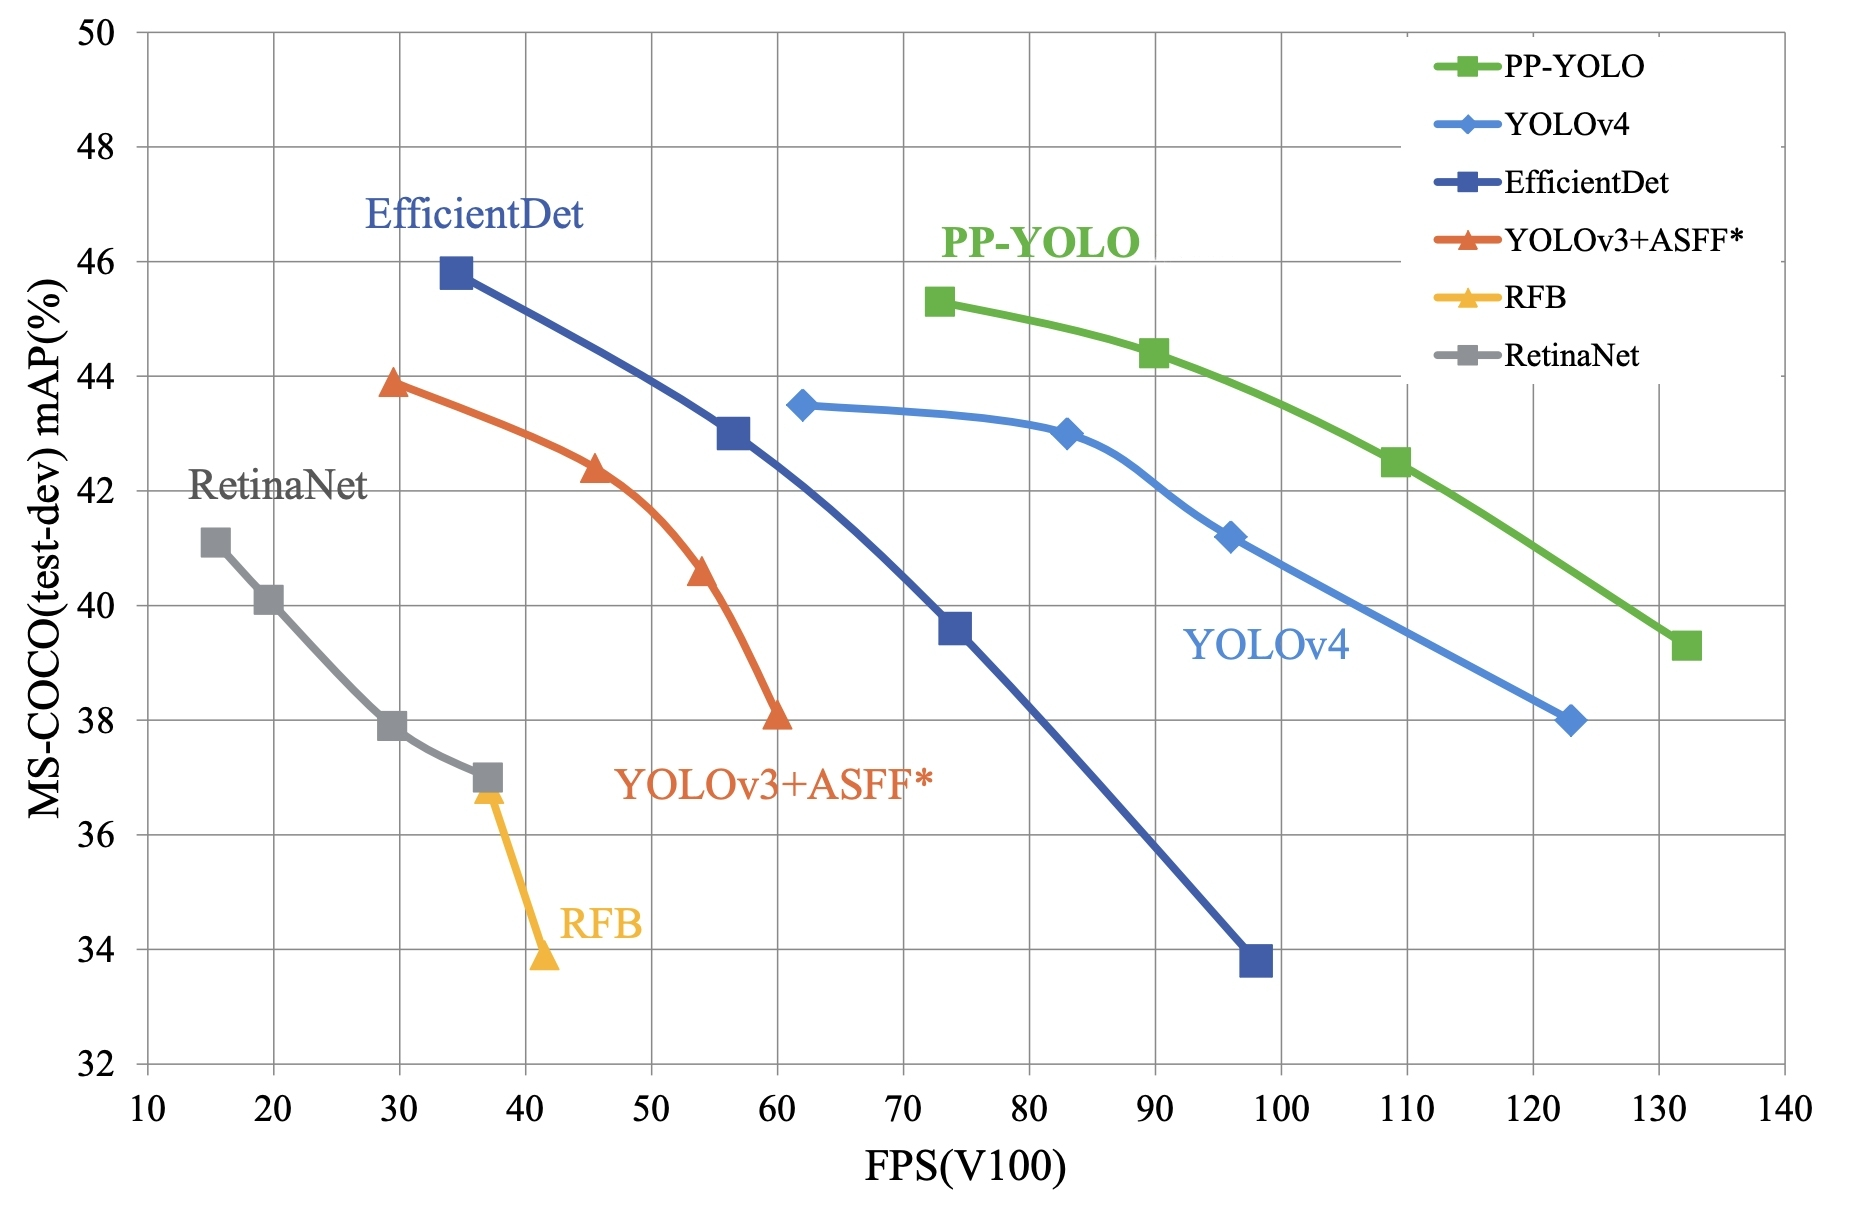
\includegraphics[width=1\columnwidth]{images/PP-YOLO.jpeg}
\caption{Comparison of the PP-YOLO and other detectors (Source: \cite{long2020pp}).}
\label{fig:pp-yolo}
\end{figure}

From Figure \ref{fig:pp-yolo}, By combining multiple tricks, Long et al. (2020) published PP-YOLO model which has an accuracy of 45.2\% and speed of 72.9 FPS in the COCO dataset, exceeding the existing state-of-the-art detectors. 
PP-YOLO does not propose a novel detection model but achieves a new object detector which can be directly applied to actual applications. Besides, PP-YOLO has achieved a balance of accuracy and speed and tried various techniques. These technologies are the goal of improving the accuracy of the detector as much as possible while ensuring that the speed is almost unchanged, and hardly increase the number of model parameters.

In terms of the backbone network, ResNet is used in PP-YOLO. One of the reasons is that ResNet has been deeply optimized and widely used, which makes its inference speed faster. Another reason is that the backbone network and the data augmentation method are relatively independent factors, and are not related to the trick of the paper's exploration. At the same time, many papers have been studied accordingly, so the author did not make relevant repeated explorations. Therefore, the author used the manual method to set the parameters along the route of YOLOv3, but the author believed that a better backbone network, a better augmentation scheme, and Neural Architecture Search (NAS) search hyperparameters can further improve the performance of PP-YOLO.


\begin{figure}[htbp]
\centering
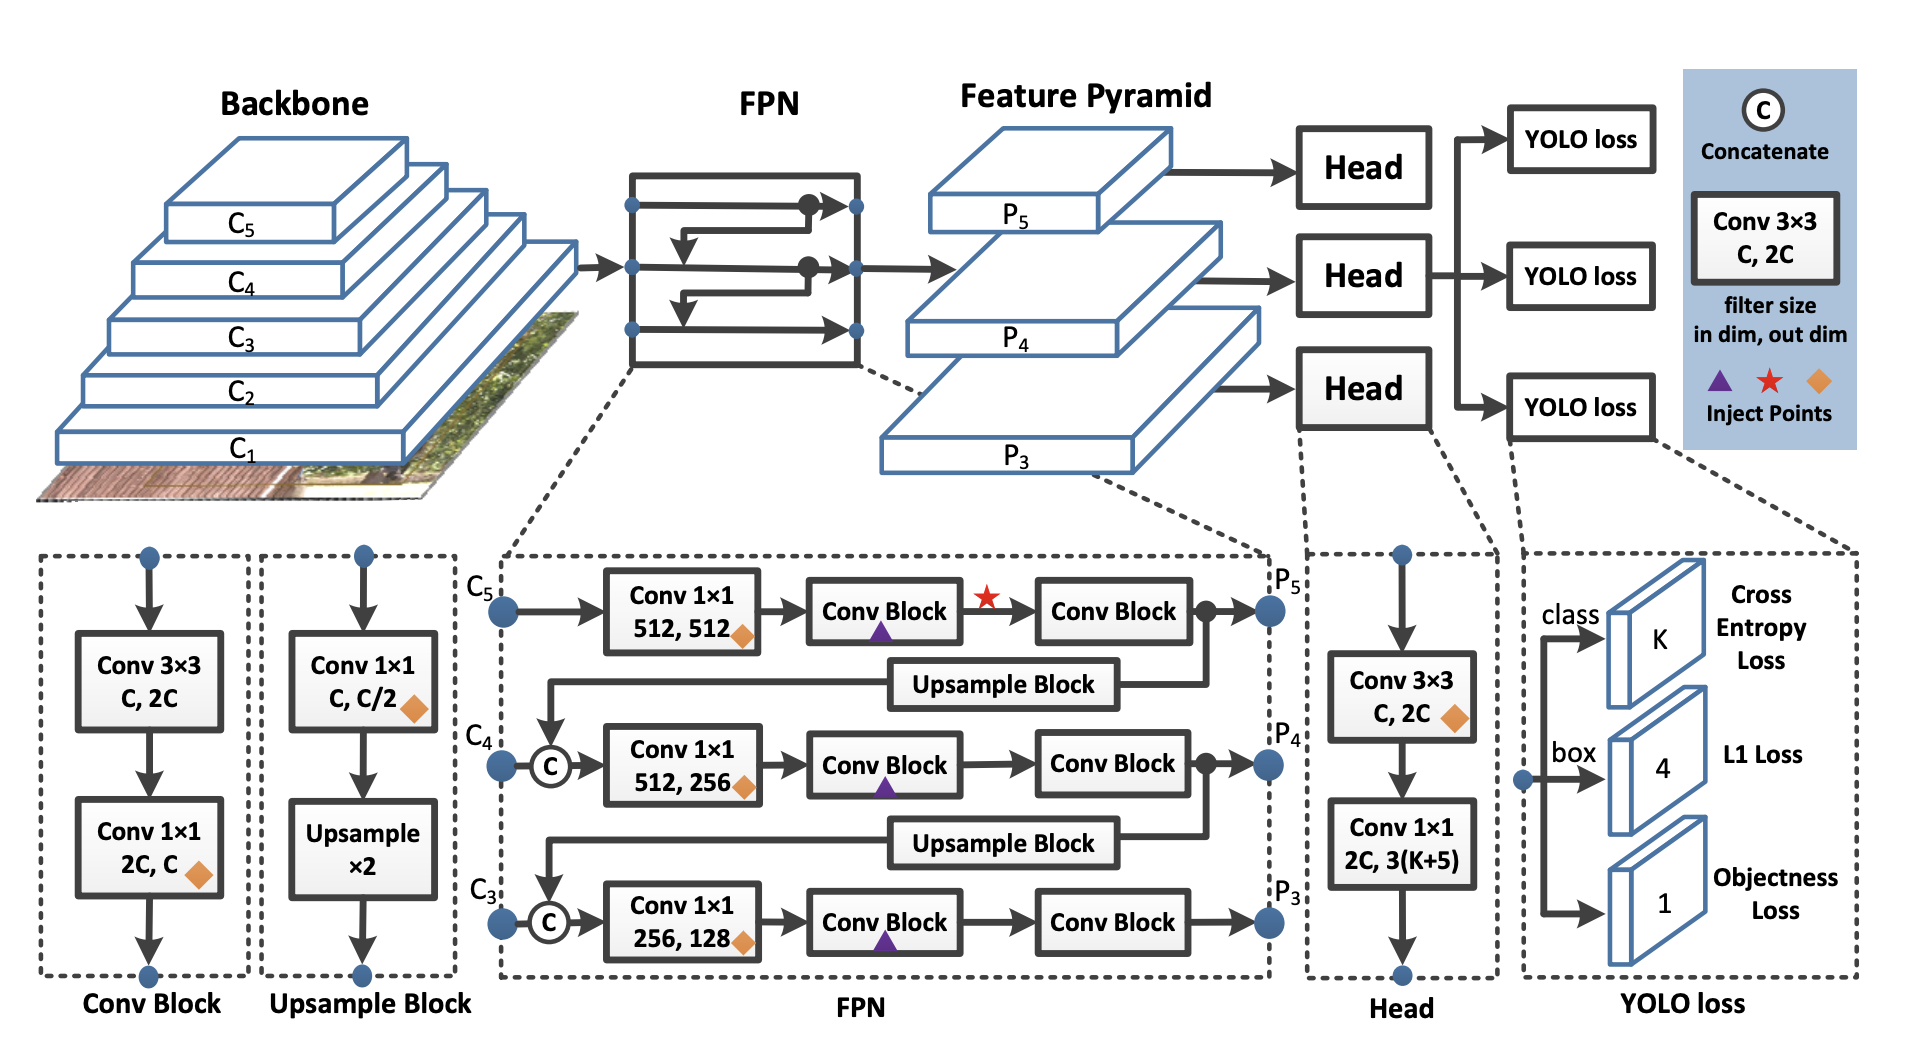
\includegraphics[width=1\columnwidth]{images/PP-YOLO architecture.png}
\caption{The network architecture of the PP-YOLO (Source: \cite{long2020pp}).}
\label{fig:network architecture}
\end{figure}

From the content of this paper and the network architecture in Figure \ref{fig:network architecture}, some technical details are found as follows.

\begin{itemize}
\item{Backbone}

Different variants of backbone networks have been explored in the last couple of years. The most efficient and popular backbone is the ResNet network which is quite a famous network architecture for object classification tasks. In the original YOLOv3 paper, the Darknet-53 architecture was used \cite{he2016deep}. However, since ResNet has been widely studied and comes bundled with pre-trained networks, the author decided to choose ResNet50 as a backbone network architecture which provides a boost in both effectiveness and efficiency.

\end{itemize}

\begin{itemize}
\item{Neck}

The neck of the network is where the network is made robust by making it scale and size invariant. The author used Feature Pyramid Networks (FPN) to construct a feature pyramid to connect features horizontally. The author selected the last three convolutional layers C3, C4, C5, and then merged the high-level semantic information with the low-level information through the FPN structure.

\end{itemize}


\begin{itemize}

\item{Head}

This is the final layer of the network which outputs the bounding box coordinates, category and confidence score of the object. The detection head includes two convolutional layers. A 3 x 3 convolutional layer and a 1 x 1 convolutional layer are used to obtain the final prediction result. For classification and positioning, cross-entropy loss and Smooth L1 loss are used accordingly, and confidence loss is used to monitor the object score and to identify whether there is an object.
\end{itemize}

The paper did not propose a new detection method but focused on combining existing detection methods to achieve an efficient detector. Since many techniques cannot be directly applied to YOLOv3, they need to be adjusted according to its structure.

\begin{table}[htbp]
\centering
\caption{The ablation study of tricks on the MS-COCO minival split (Source: \cite{long2020pp}).}
\begin{tabular}{lp{3cm}<{}lllll} 
\toprule
\textbf{Group}&\textbf{Methods}&\textbf{mAP}&\textbf{Parameters}&\textbf{GFLOPs}&\textbf{infer time}&\textbf{FPS}\\
\midrule
A& Darknet53 YOLOv3 &38.9 & 59.13 M& 65.52 & 17.2 ms &58.2\\
\cmidrule(r){1-7}
B& ResNet50-vd-dcn YOLOv3 &39.1 & 43.89 M & 44.71 & 12.6 ms & 79.2\\
C& B + LB + EMA + DropBlock& 41.4 & 43.89 M & 44.71 & 12.6 ms &79.2\\
D& C + IoU Loss& 41.9 & 43.89 M & 44.71 & 12.6 ms &79.2\\
E& D + IoU Aware & 42.5 & 43.90 M & 44.71 & 13.3 ms &74.9\\
F& E + Grid Sensitive& 42.8 & 43.90 M & 44.71 & 13.4 ms &74.8\\
G& F + Matrix NMS& 43.5 & 43.90 M & 44.71 & 13.4 ms &74.8\\
H& G + CoordConv& 44.0 & 43.93 M & 44.76 & 13.5 ms &74.1\\
I& H + SSP& 44.3 & 43.93 M & 45.12 & 13.7 ms &72.9\\
J& I + Better ImageNet Pretrain& 44.6& 43.93 M & 45.12 & 13.7 ms& 72.9\\
\bottomrule
\end{tabular}
\label{tbl:ablation study pp-yolo}
\end{table}

Table \ref{tbl:ablation study pp-yolo} shows the comparison of the mAP, parameters, FLOPs, infer time and FPS produced by different tricks. The results indicate that by using different combinations, PP-YOLO can achieve performance improvements.

Although PP-YOLO has dramatically improved in speed and accuracy, it has not done more experiments on the backbone, FPN, data augmentation and NAS. Therefore, these aspects can be studied to improve the effectiveness of the detector.



\subsection{Model Improvement Skills}
\subsubsection{Transfer Learning}

When training a deep learning model, a large number of data is usually required. However, data preparation processes such as data collection and labeling will cost a lot in labor and time.
Pan and Yang (2009) proposed transfer learning in which that we can choose to train a convergent and effective model on an extensive public data set as the pre-training weight and use business data to fine-tune the model on this basis \cite{pan2009survey}.

Zhuang et al. (2020) reviewed a variety of representative transfer learning methods from the perspective of data and models, especially similar transfer learning methods \cite{zhuang2020comprehensive}. He also briefly introduced the application of transfer learning.
Inspired by their ideas, we can use a large number of knowledge reserves of the pre-training model to quickly and efficiently train a model with excellent performance for specific business scenarios.


\subsubsection{Backbone}

\begin{itemize}
\item ResNet50
\end{itemize}

ResNet is the abbreviation of Residual Network proposed by He et al. (2016) \cite{he2016deep}. ResNet solved the problems of gradient dispersion and accuracy drop in the deep network so that the network can get deeper and deeper, which not only ensures the accuracy but also controls the speed. ResNet first performs a convolution operation on the input, and then contains four residual blocks and finally performs a fully connected operation to facilitate classification tasks. The network composition diagram is presented in Table \ref{tbl:ResNet}.


\begin{table}[htbp]
\centering
\caption{Structure of ResNet (Source: \cite{he2016deep}).}
\begin{tabular}{c|c|c|c|c|c}
\hline
\textbf{layer name}                & \textbf{output size}    & \textbf{18-layer} & \textbf{34-layer} & \textbf{50-layer} & \textbf{101-layer}  \\ \hline
\textbf{conv1}                     & 112$\times$112               & \multicolumn{4}{c}{7$\times$7, 64, stride 2}                                                              \\ \hline
\multirow{2}{*}{\textbf{conv2\_x}} & \multirow{2}{*}{56$\times$56} & \multicolumn{4}{c}{3$\times$3 max pool, stride 2}                                                         \\ \cline{3-6}  &   &$\begin{bmatrix} 3\times3, 64 \\  3\times3, 64 \\  \end{bmatrix}\times2$&
$\begin{bmatrix}  3\times3, 64 \\  3\times3, 64 \\  \end{bmatrix}\times3$& $\begin{bmatrix}1\times1, 64 \\  3\times3, 64 \\1\times1, 256 \\  \end{bmatrix}\times3$ 
& $\begin{bmatrix}  1\times1, 64 \\  3\times3, 64 \\1\times1, 256 \\    
\end{bmatrix}\times3$                               \\ \hline
\textbf{conv3\_x}  & 28$\times$28 & $\begin{bmatrix}  3\times3, 128 \\  3\times3, 128 \\ \end{bmatrix}\times2$&$\begin{bmatrix}  3\times3, 128 \\  3\times3, 128 \\  \end{bmatrix}\times4$& $\begin{bmatrix}  1\times1, 128 \\  3\times3, 128 \\1\times1, 512 \\      \end{bmatrix}\times4$ & $\begin{bmatrix}  1\times1, 128 \\  3\times3, 128 \\1\times1, 512 \\    
\end{bmatrix}\times4$ \\ \hline\textbf{conv4\_x}    & 14$\times$14       & $\begin{bmatrix} 3\times3, 256 \\  3\times3, 256 \\    \end{bmatrix}\times2$
&$\begin{bmatrix}  3\times3, 256 \\  3\times3, 256 \\    \end{bmatrix}\times6$
& $\begin{bmatrix}  1\times1, 256 \\  3\times3, 256 \\1\times1, 1024\end{bmatrix}\times6$ 
& $\begin{bmatrix}  1\times1, 256 \\  3\times3, 256 \\1\times1, 1024 \\    
\end{bmatrix}\times23$      \\ \hline
\textbf{conv5\_x}     & 7$\times$7   & $\begin{bmatrix}  3\times3, 512 \\  3\times3, 512 \\    
\end{bmatrix}\times2$&$\begin{bmatrix}  3\times3, 512 \\  3\times3, 512 \\    
\end{bmatrix}\times3$
& $\begin{bmatrix}  1\times1, 512 \\  3\times3, 512 \\1\times1, 2048 \\      
\end{bmatrix}\times3$ & $\begin{bmatrix}  1\times1, 512 \\  3\times3, 512 \\1\times1, 2048 \\    
\end{bmatrix}\times3$   \\ \hline
\textbf{}    & 1$\times$1   & \multicolumn{4}{c}{average pool, 1000-d fc, softmax}                                             \\ \hline\multicolumn{2}{c|}{\textbf{FLOPs}}  & $1.8\times10^{9}$ & $3.6\times10^{9}$ &$3.8\times10^{9}$ & $7.6\times10^{9}$  \\ \hline
\end{tabular}
\label{tbl:ResNet}
\end{table}

From the column named 50-layer, ResNet50 has four large blocks, each containing 3, 4, 6, and 3 small blocks. There are three convolutions in each small block. In addition, the network has two layers at the beginning and the end, a single convolutional layer and a fully connected layer. Therefore, a total of 50 layers ((3 + 4 + 6 + 3) * 3 + 1 + 1 = 50) are included in ResNet50.


\begin{itemize}
\item MobileNetV2
\end{itemize}

Mobile Network (MobileNet) is a lightweight visual architecture suitable for embedded devices proposed by Sandler et al. (2018) from Google \cite{sandler2018mobilenetv2}. The purpose of this model is to ensure the efficiency of use on mobile devices. MobileNet has the advantages of a few parameters and simple structure, and can be used in computer vision applications such as classification and detection.

The structure of MobileNetV2 is based on inverted residual, which is essentially a residual network. The traditional residual block has a large number of channels at both ends of the block and a small number in the middle, while the inverted residual is that the number of channels at both ends of the block is small, and there are many channels in the block.


\begin{table}[htbp]
\centering
\caption{Structure of MobileNetV2 (Source: \cite{sandler2018mobilenetv2}).}
\begin{tabular}{llllll} 
\toprule
\textbf{Input}&\textbf{Operator}&\textbf{$t$}&\textbf{$c$}&\textbf{$n$}&\textbf{$s$}\\
\midrule
$224^2$ $\times$ 3&3conv2d & - & 32 & 1 & 2\\
$112^2$ $\times$ 32& bottleneck & 1 & 16 & 1 &1\\
$112^2$ $\times$ 16& bottleneck & 6 & 24 & 2 &2\\
$56^2$ $\times$ 24& bottleneck & 6 & 32 & 3 &2\\
$28^2$ $\times$ 32& bottleneck & 6 & 64 & 4 &2\\
$14^2$ $\times$ 64& bottleneck & 6 & 96 & 3 &1\\
$14^2$ $\times$ 96& bottleneck & 6 & 160 & 3 &2\\
$7^2$ $\times$ 160& bottleneck & 6 & 320 & 1 &1\\
$7^2$ $\times$ 320& conv2d 1 $\times$ 1 & - & 1280 & 1 &1\\
$7^2$ $\times$ 1280& avgpool 7 $\times$ 7& - & - & 1& 1\\
1 $\times$ 1 $\times$ 1280& conv2d 1 $\times$ 1& - & k & - & \\
\bottomrule
\end{tabular}
\label{tbl:MobileNetV2}
\end{table}



As can be seen from Table \ref{tbl:MobileNetV2}, the input image resolution of the classification network structure shown in the figure is 224 $\times$ 224. The primary unit bottleneck is the inverted residuals module. The output is full convolution instead of softmax, and $k$ is the number of categories of the recognition target.

MobileNetV2 uses depth-wise (DW) convolution and point-wise (PW) convolution to extract features. The combination of these two operations is also called Depth-wise Separable Convolution, which was widely used in Xception before \cite{sandler2018mobilenetv2}. The advantage is that in theory, the time complexity and space complexity of the convolutional layer can be reduced.

\subsubsection{Data Augmentation}

The data augmentation technology generates similar but different training samples by making a series of random changes to the training images, thereby expanding the size of the training dataset. Frid-Adar et al. (2018) proposed that the commonly used image augmentation techniques are mirror transformation, rotation, zooming, cropping, translation, brightness modification, noise adding, cutting, and color changing \cite{frid2018gan}.

Compared with the above-mentioned standard image augmentation methods, researchers have also proposed many improved image augmentation strategies, like mixup, random distort, random expand, etc. \cite{cubuk2018autoaugment, devries2017improved}. These strategies are all inserting certain operations at different stages of the standard augmentation method. Through these methods, the diversity of samples is increased. If we apply these methods to our experiments, more complex situations can be handled and complex water obstacles can be detected.

\subsection{Summary}

From the literature described above, it can be found that the obstacle detection of USVs does present significant challenges. A vision-based sensor like a camera is a suitable solution because it can not only perceive obstacles but also know the appearance of obstacles. The PP-YOLO algorithm is currently a fast and accurate algorithm, which can be applied to the obstacle recognition of USVs. Some model improvement techniques, such as 
backbone replacement, data augmentation can be applied to the PP-YOLO, which may increase model accuracy and speed.

\section{System Design}

\begin{figure}[htbp]
\centering
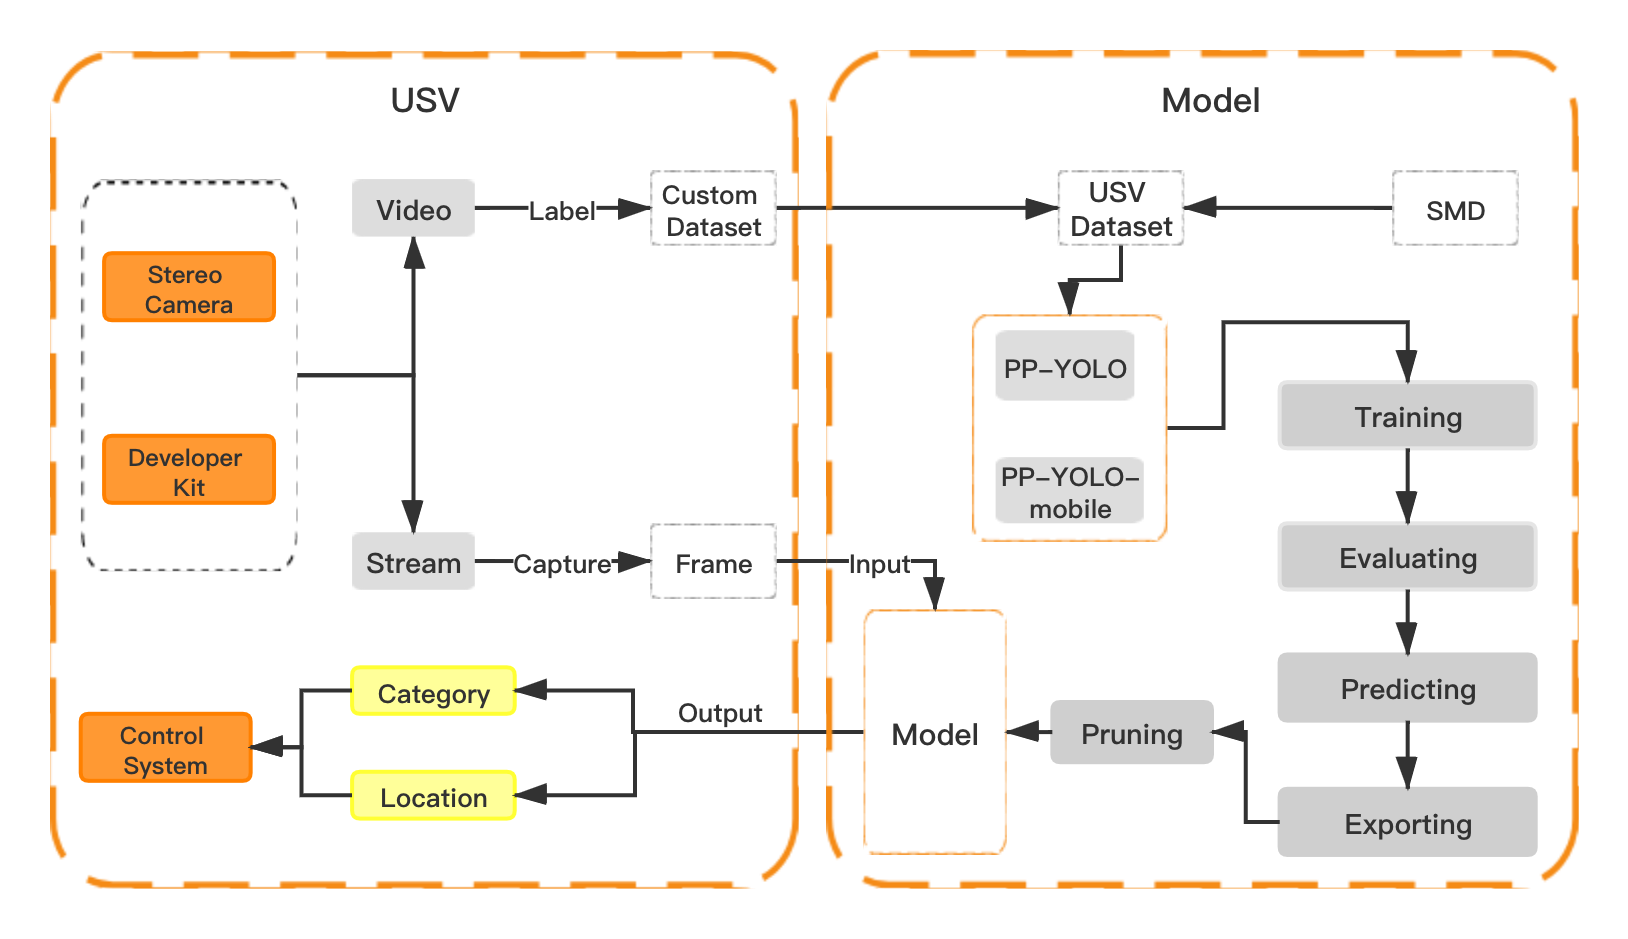
\includegraphics[width=0.8\textwidth]{images/design.png}
\caption{System design diagram.}
\label{fig:system architecture}
\end{figure}

As can be vividly seen from Figure \ref{fig:system architecture}, the system design mainly includes two parts, one is the deployment and data processing of the USV, and the other is the implementation of the PP-YOLO model and  PP-YOLO-mobile model. The stereo camera and the developer kit are used to obtain the video data for custom dataset labeling and real-time obstacle detection. The USV dataset is composed of the custom dataset and the Singapore Maritime Dataset (SMD). Both the PP-YOLO model and the PP-YOLO-mobile model are constructed through training, evaluating, predicting and exporting. The completed model is then pruned to reduce the size and deployed on a developer kit for identifying the obstacles from the video stream. Location and category of the obstacle are predicted and sent to the control system for obstacle avoidance.


\subsection{USV Construction}
\begin{figure}[htbp]
\centering
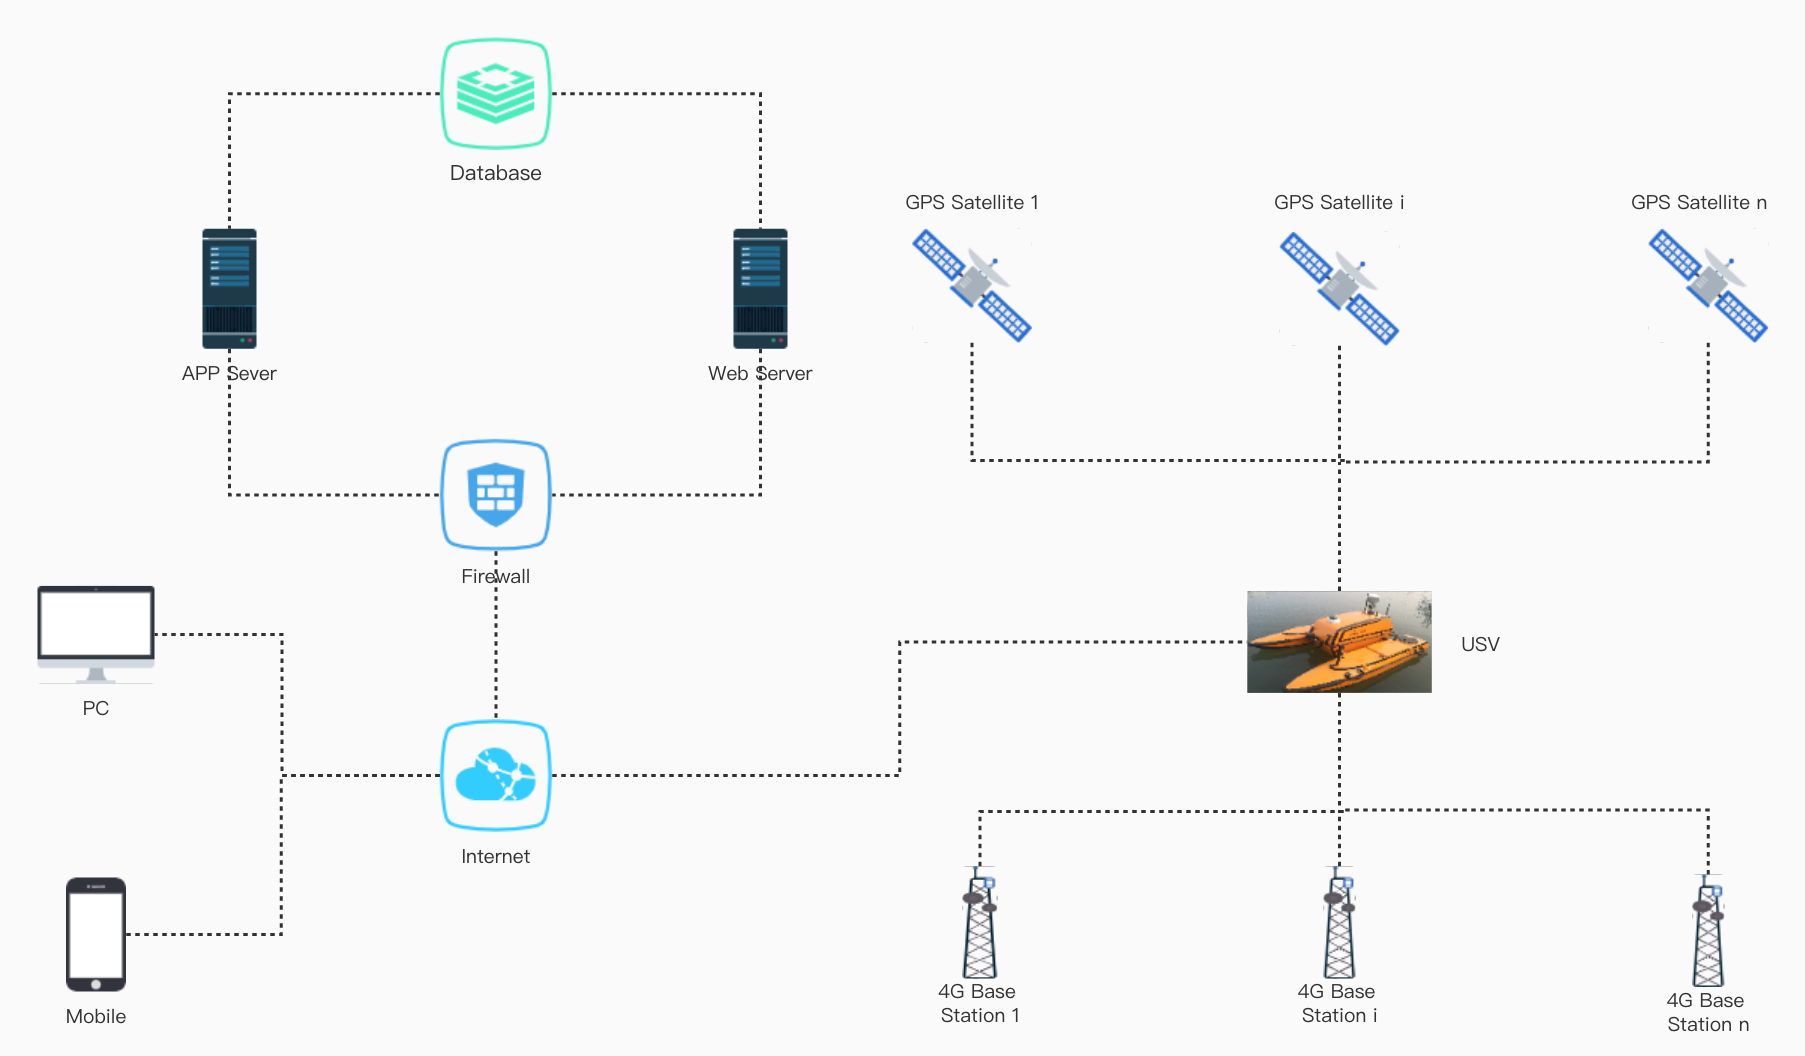
\includegraphics[width=1\columnwidth]{images/USV-architecture.jpg}
\caption{Architecture of the USVs}
\label{fig:Architecture of USVs}
\end{figure}

The architecture of the USV is shown in Figure \ref{fig:Architecture of USVs}. The Global Positioning System (GPS) signal receiver is installed on the USV to obtain the longitude and latitude information of its own position. The Inertial Measurement Unit (IMU) is used to obtain acceleration and velocity information of the USV in real-time.

A stereo camera and developer kit are installed in the cabin for detecting and recognizing the obstacles. When an obstacle is found from the signal of the stereo camera, the deployed model will calculate the location by drawing a bounding box and identify the category of this obstacle. After that, it can send instructions to control the heading and speed of the USV so that it can avoid the obstacle.

Sensors for water quality measurement are deployed under the hull to collect the water quality data at regular intervals. The data can be transmitted to the back-end server through the 4G-based Data Transmission Unit (DTU). Application Programming Interface (API) deployed on the server receives the request and saves the water quality data in the database after processing. Users can view water quality data and analysis reports on the web browser or the mobile application.



\subsection{Model Construction}

The construction of the models is based on an open-source deep learning platform derived from industry practice called PaddlePaddle, which aims to make the innovation and application of deep learning technology easier \cite{ma2019paddlepaddle}.
PaddleX is a full-process development tool for PaddlePaddle, which integrates all the capabilities required for deep learning development such as the core framework of PaddlePaddle, model libraries, tools and components. PaddleX also provides a concise and easy-to-understand Python API, and a graphical development client for one-click download and installation. Users can choose the corresponding development method according to actual production needs, and get the best experience of the whole process of PaddlePaddle development. AIStudio is a platform for deep learning which provides an online programming environment, free GPU services, massive open-source algorithms and open data to help developers quickly create and deploy models. 
With the help of the above services, the model construction of this experiment is easier to complete.

\subsubsection{PP-YOLO Model}

According to the instruction provided by Long et al. (2020) \cite{long2020pp}, construction of the PP-YOLO model requires the following steps:

\begin{enumerate}
\item Training PP-YOLO model after configuring some parameters.
\item Saving and evaluating the model on the validation set.
\item Inferring on the testing set and outputting the location and category of the target.
\item Exporting the best model and using PaddlePaddle prediction library for predicting.
\end{enumerate}

\subsubsection{PP-YOLO-mobile Model}

In order to adapt to the scene of avoidance for USVs, 
some improvements need to be done. By referring to the methods from \cite{zoph2019learning, mahto2020refining, mandal2020object}, two improvements have been made in this research, namely backbone replacement and data augmentation.

\begin{itemize}
\item{Backbone Replacement}

\begin{figure}[htbp]
\centering
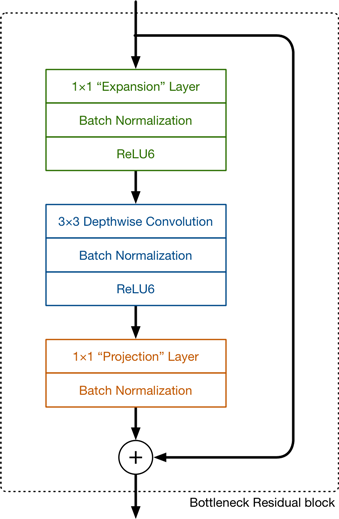
\includegraphics[width=0.45\columnwidth]{images/MobileNetV2-structure.png}
\caption{Network of MobileNetV2.}
\label{fig:Microstructure}
\end{figure}

In the MobileNet, Depth-wise Separable Convolution is introduced, which dramatically reduce the complexity cost and model size of the network. The PP-YOLO-mobile model uses MobileNetV2 as the backbone to extract information features from the input image, which is suitable for low-power embedded devices.



In the network design of MobileNetV2 in Figure \ref{fig:Microstructure}, the author not only continued to use the Depth-wise Separable Convolution but also Expansion layer and Projection layer. This projection layer uses a 1 x 1 network structure, and its purpose is to map high-dimensional features to low-dimensional space. In addition, the network uses a 1 x 1 network structure to map high-dimensional space to low-dimensional space is also called the Bottleneck layer.

In contrast to the projection layer, the expansion layer uses a 1 x 1 network structure to map the low-dimensional space to the high-dimensional space. The expansion has a hyperparameter that expands the dimension several times, which can be adjusted according to the actual situation. The default value is 6, which means the expansion is 6 times.



\end{itemize}

\begin{itemize}
\item{Data Augmentation}


Since all the data comes from videos of the USV when sailing, the source of the data is relatively simple and cannot cover various environments. Besides, obstacles on the river surface will be affected by light exposure and river fluctuations. Therefore, the appearance of the same obstacle at different times is different, which also brings difficulty to obstacle detection. In order to recognize obstacles under different conditions, the model needs to deal with the influence of different lighting, background environment and other noises.

The data augmentation operation is used to increase the diversity of dataset during model training, thereby enhancing the ability of generalisation. In this research, data augmentation expands the dataset of river obstacles by including brightness transformation, contrast enhancement, sharpening, etc. The following data augmentation methods are used in this experiment:



\begin{itemize}
\item{Mixup}

Mixup is a technique similar to regularization, which interpolates data in a high-dimensional space, increases the size of the pseudo-data set, and reduces the overfitting of the model to a certain extent. 
\end{itemize}


\begin{itemize}
\item{Random Distort}

Random distort performs random pixel content transformation on the image with a certain probability, including brightness, contrast, saturation and hue.

\end{itemize}

\begin{itemize}
\item{Random Expand}

Random expand randomly selects the expansion ratio to expand the image. Firstly, it calculates the image size after expansion. Then, it initializes the pixel value of the image with the input fill value and pastes the original image on the image randomly. Finally, according to the original image pasting position, it converts the position coordinates of the real label frame after expansion.

\end{itemize}


\begin{itemize}
\item{Random Crop}

 It randomly crops the image through the following steps. Firstly, it calculates the height and width of a random crop. Then it randomly selects the starting point of the crop according to the height and width of the random crop. After the final cropping is completed, it adjusts the image to a uniform size.

\end{itemize}


\begin{itemize}
\item{Resize}

This step adjusts the image to a uniform length and width of 608 pixels to meet the requirements of model input size.

\end{itemize}


\begin{itemize}
\item{Random Horizontal Flip}

This method randomly flips the image horizontally with a certain probability.

\end{itemize}
\end{itemize}


\subsection{Ablation Study}
Although both backbone replacement and data augmentation may improve the model, the experiment did not prove that the two methods are meaningful, respectively. Meyes et al. (2019) proposed that an ablation study typically refers to removing some features of the model or algorithm, and seeing how that affects performance \cite{meyes2019ablation}.
Inspired by his idea, we changed multiple methods at the same time by controlling the method one by one to find which method have a more significant impact on the results. Table \ref{tbl:design of ablation study for PP-YOLO} shows the design of the ablation study.

\begin{table}[htbp]
\centering
\caption{Design of ablation study for PP-YOLO}
\begin{tabular}{ll} 
\toprule
\textbf{Group}&\textbf{Methods}\\
\midrule
A& PP-YOLO + ResNet50 (Benchmark) \\
\cmidrule(r){1-2}
B& PP-YOLO + MobileNetV2 \\
C& PP-YOLO + ResNet50 + Data Augmentation \\
D& PP-YOLO + MobileNetV2 + Data Augmentation\\
\bottomrule
\end{tabular}
\label{tbl:design of ablation study for PP-YOLO}
\end{table}


\begin{itemize}
\item{Group A is the original PP-YOLO model, using the ResNet50 backbone, which is also the benchmark for this experiment.}
\end{itemize}


\begin{itemize}
\item{Group B is replaced with MobileNetV2 backbone based on Group A, which is used to compare the performance of the two backbone with Group A.}
\end{itemize}

\begin{itemize}
\item{Group C adds data augmentation methods based on Group A. When comparing the experimental results with group A, we can find that how effective data enhancement is worked on the model.}
\end{itemize}

\begin{itemize}
\item{Group D is the PP-YOLO-mobile model, which adds data augmentation based on Group B. Comparing the experimental results with group A, we can obtain the result of adding backbone replacement and data augmentation to the model at the same time.}
\end{itemize}


\section{Implementation}
\subsection{Data Collection}

\subsubsection{Singapore Maritime Dataset}
The Singapore Maritime Dataset (SMD) is a set of videos of the sea surface from Singapore captured by Dilip K. Prasad and volunteers using a Canon 70D camera \cite{prasad2017video}. All the videos are acquired in high definition (1080 $\times$ 1920 pixels) and are divided into three types, on-shore videos, on-board videos and Near Infra Red (NIR) videos. From the contents of the videos, they cover not only different time periods, such as before sunrise, sunrise, noon, afternoon, evening, and after sunset, but also include different weather conditions, like sunny, haze, and rain. Totally, there are 81 videos with nine different categories and 240,842 object labels in this dataset. Figure \ref{fig:Simple images of the SMD} displays simple images of the dataset and Table \ref{tbl:Properties of Singapore Maritime Dataset} summarizes the properties of each type of video in the dataset.


\begin{figure}[htbp]
\centering
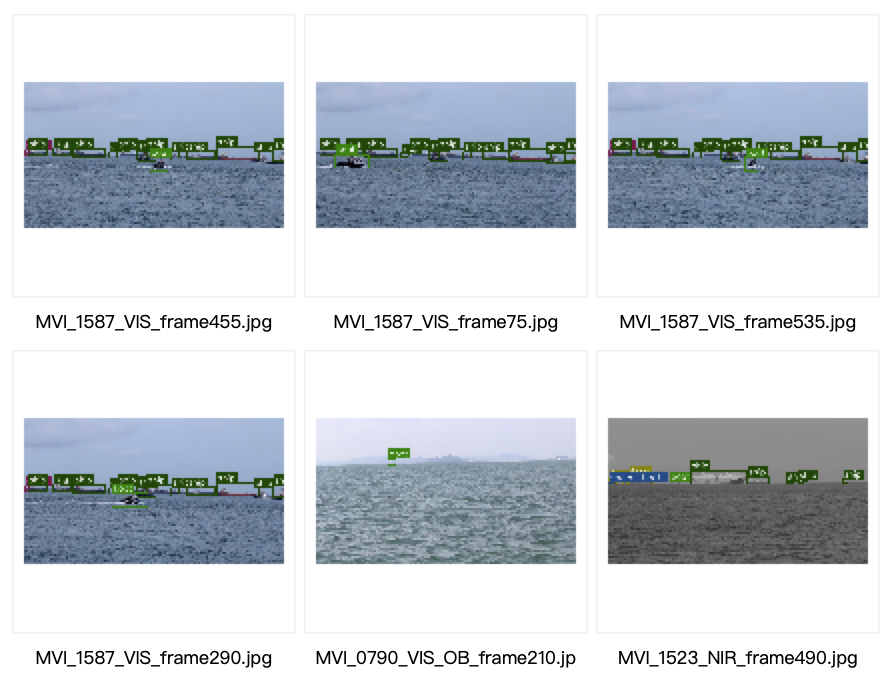
\includegraphics[width=1\columnwidth]{images/SMD-example.png}
\caption{Simple images of the SMD.}
\label{fig:Simple images of the SMD}
\end{figure}

\begin{table}[htbp]
\centering
\caption{Properties of the Singapore Maritime Dataset.}
\begin{tabular}{llllll} 
\toprule
\textbf{Sub dataset}&\textbf{Size}&\textbf{All Videos}&\textbf{Annotated Videos}&\textbf{Labelled Frames}& \textbf{Labels}\\
\midrule
On-Shore & 3 GB& 40 & 36 & 17,967& 154,495\\
On-Board & 768 MB&  11 &4 &2,400& 3,173\\
NIR& 1.51 GB&  30&23 & 11,286& 83,174\\
\cmidrule(r){1-6}
Total& 5.28 G&  81 &63 & 31,653 &240,842\\
\bottomrule
\end{tabular}
\label{tbl:Properties of Singapore Maritime Dataset}
\end{table}


\subsubsection{Custom Dataset}

Since the SMD are focused on objects from the sea surface, obstacles on rivers are not provided, such as water plants and floating garbage. To achieve the function of guiding the USVs to detect the obstacles, dataset needs to be expanded with more kinds of obstacles.

The custom dataset consists of two parts, one is the video data collected by a camera deployed on the USV during its navigation, and the other is the images of the river surface retrieved from the Internet. Labeling tool named LabelMe is used to label the images by drawing rectangular boxes and selecting corresponding labels. The location and classification information of each marked object in the image is saved in a JSON format file. Figure \ref{fig:Simple images of the custom dataset} shows some images from the custom dataset. 

\begin{figure}[htbp]
\centering
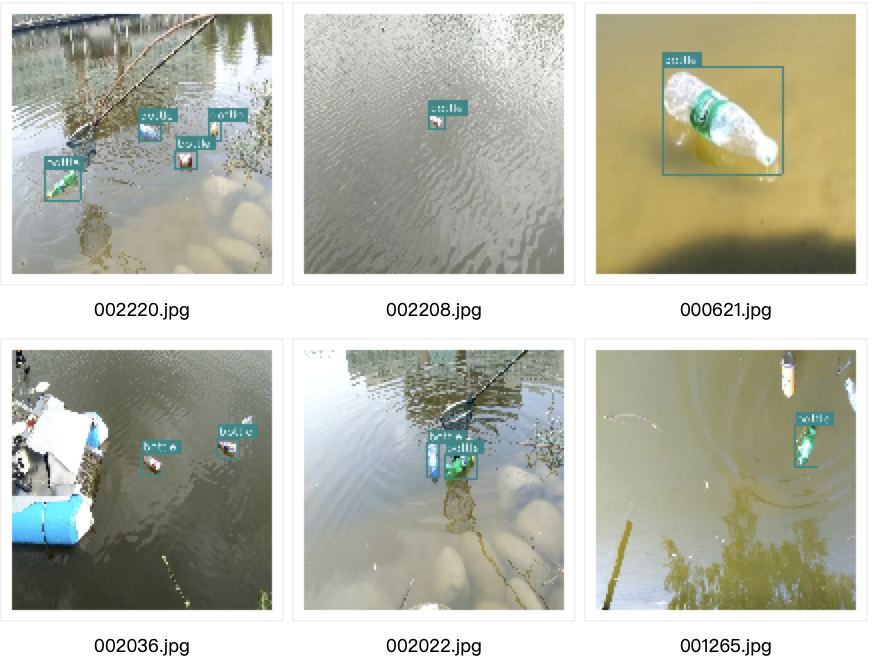
\includegraphics[width=1\columnwidth]{images/custom-dataset-example.png}
\caption{Simple images of the custom dataset.}
\label{fig:Simple images of the custom dataset}
\end{figure}


\subsubsection{USV Dataset}
After the custom dataset is all marked, it is merged with the SMD to form the USV dataset. Finally, the USV dataset contains 17 categories and a total of 8,750 images. In the dataset, common obstacles on the river surface are included, such as various boats, buoys, bottles, and water plants, which can meet the data preparation for obstacle detection and recognition.

In order to perform training, the dataset is divided into a training set, validation set and testing set according to the ratio of 7 : 2 : 1. The number of various categories in different sets is described in Table \ref{tbl:USV dataset for obstacle detection}.

\begin{table}[htbp]
\centering
\caption{USV dataset for obstacle detection}
\begin{tabular}{llllll} 
\toprule
\textbf{Category}&\textbf{Total Number}&\textbf{Training}&\textbf{Validation}&\textbf{Testing}\\
\midrule
ball& 49& 32& 12& 5 \\
boat& 350& 240& 75& 35 \\
bottle& 1,039& 742& 193& 104 \\
branch& 404& 279& 78& 47 \\
buoy& 567& 380& 121& 66 \\
ferry& 1,572& 1,095& 339& 138 \\
flying-bird& 194& 128& 43& 23 \\
grass& 201& 139& 44& 18 \\
kayak& 200& 133& 44& 23 \\
leaf& 248& 177& 38& 33 \\
milk-box& 233& 169& 45& 19 \\
other& 2,936& 2,064& 611& 261 \\
plastic-bag& 393& 284& 72& 37 \\
plastic-garbage& 192& 145& 31& 16 \\
sail-boat& 616& 406& 138& 72 \\
ship& 6180& 4,284& 1,278& 618 \\
speed-boat& 1,535& 1,030& 336& 169 \\
\cmidrule(r){1-5}
Total& 8,750& 6,125& 1,750& 875 \\
\bottomrule
\end{tabular}
\label{tbl:USV dataset for obstacle detection}
\end{table}



\subsubsection{Data Processing}
\begin{figure}[htbp]
\centering
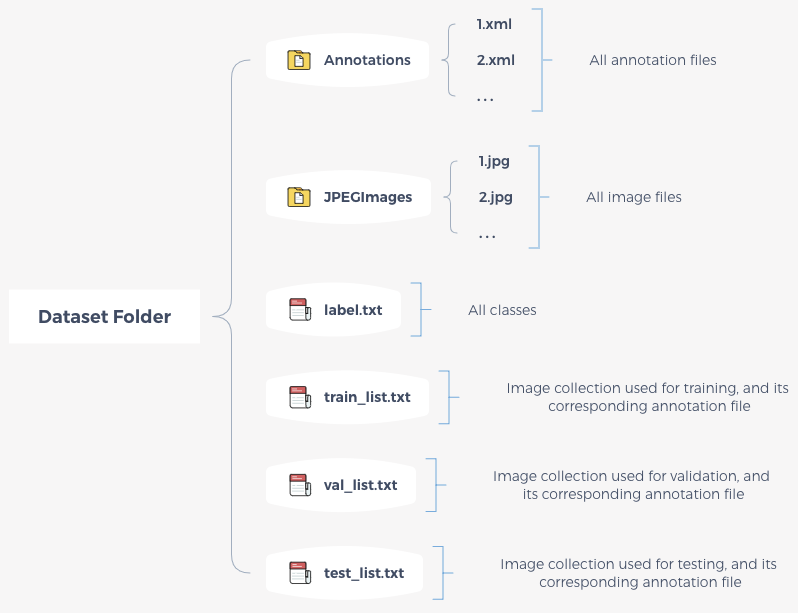
\includegraphics[width=1\columnwidth]{images/dataset-folder.png}
\caption{Structure of the dataset folder.}
\label{fig:Structure of the dataset folder}
\end{figure}

As the standard format for object detection is PascalVOC with XML format, the labeled data needs to be converted to that format using python script. The information of all targets in each image are recorded, including the pixel positions of the four vertices, the name of the target category and the path where the picture is located.
Besides, image files and annotation files need to be stored in their respective folders named JPEGImages and Annotation. There is also one text file recording all the 17 categories and three text files for image lists of training, validation and testing.

After those processes, the complete USV dataset is finished. When the model starts training, the dataset can be directly loaded. The structure of the dataset folder is shown in Figure \ref{fig:Structure of the dataset folder}.


\subsection{Model Implementation}

\subsubsection{Hardware Environment}

Table \ref{tbl:Hardware} shows the hardware environment for the model training, including 4-core CPU, 32G memory, 100G hard disk. A Tesla V100 graphics card is equipped in the server with a memory of 16GB. Furthermore, the operating system of this server is Ubuntu 18.04.

\begin{table}[htbp]
\centering
\caption{Hardware environment of the training server}
\begin{tabular}{ll} 
\toprule
\textbf{Name}&\textbf{Configuration}\\
\midrule
CPU& 4 Core \\
RAM& 32 GB \\
GPU& Tesla V100 \\
Video Memory& 16 GB\\
Disk& 100 GB\\
Operating System& Ubuntu 18.04\\
\bottomrule
\end{tabular}
\label{tbl:Hardware}
\end{table}

The above configuration has met the requirements of model training. Besides, all models are trained in the above configuration to ensure the consistency of the experimental environment.

\subsubsection{Model Configuration}

Table \ref{tbl:Parameter} shows the parameter configuration of the PP-YOLO model and the PP-YOLO-mobile model. As can be seen from the table, the difference between the two models is the backbone and data augmentation. The backbone used in the PP-YOLO model is ResNet50 while in the PP-YOLO-mobile model is MobileNetV2. The PP-YOLO-mobile model uses data augmentation while PP-YOLO mobile does not. These two parts are the independent variables of this experiment, and the dependent variable is the trained model.

\begin{table*}[htbp]
\centering
\caption{Comparison of parameter configuration}
\begin{tabular}{llll} 
\toprule
\multicolumn{2}{l}{\textbf{Parameter Name}}&\textbf{PP-YOLO}&\textbf{PP-YOLO-mobile}\\
\midrule
\multicolumn{2}{l}{Backbone} & ResNet50 & MobileNetV2 \\
\multicolumn{2}{l}{Pre-train Model} & COCO & COCO \\
\cmidrule(r){1-4}

\multirow{1}{*}{Model Parameter} 
& Input Size & 608 x 608 pixel  & 608 x 608 pixel  \\
% & GPU & Nvidia Quadro P5000 & Nvidia Quadro P5000 \\
\cmidrule(r){1-4}

\multirow{6}{*}{Training Parameter} 
& Epoch& 300  & 300  \\
& Learning Rate & 0.000125 & 0.000125  \\
& Batch Size & 8 & 8 \\
& Saving Interval & 10 & 10 \\
& Warmup Start Learning Rate & 0.0 & 0.0 \\
& Warmup Steps & 1000 & 1000 \\
\cmidrule(r){1-4}

\multirow{6}{*}{Data Augmentation} 
& Mixup& No  & Yes  \\
& Random Distort & No & Yes  \\
& Random Expand & No & Yes \\
& Random Crop  & No & Yes \\
& Resize & No & Yes \\
& Random Horizontal Flip & No & Yes \\

\bottomrule
\end{tabular}
\label{tbl:Parameter}
\end{table*}

\subsubsection{Model Training}

 As the category of the custom dataset overlaps with the COCO dataset, most of the features in the new task can be learned by the pre-trained model in the old task. Then the weights trained on the COCO data set by PP-YOLO can be used for transfer learning in this experiment with a small amount of data. The premise of transfer learning is that the weight of the model can be borrowed from a model pre-trained on a similar task, and then fine-tuned on a specific task. PaddleX has provided a PP-YOLO object detection model, which can be used to train a model by configuring some training parameters.

\begin{itemize}
\item{$num\_epochs$}

$num\_epochs$ is the total number of model training iterations. In the beginning, we set a considerable value of 500 for $num\_epochs$, and judge whether the model converges according to the index performance of the model iteration process on the validation dataset. In addition, the $early\_stop$ strategy in the train interface can also be used. The model will automatically determine whether the model has converged and automatically stop during the training process.

\end{itemize}

\begin{itemize}
\item{$batch\_size$}

Batch size refers to the number of samples used for forwarding calculation once during the training process. Batch size is highly related to the video memory or memory of the machine. The higher the $batch\_size$, the higher the video memory or memory consumed. For the single GPU operating environment of this experiment, $batch\_size$ is set to 8.
\end{itemize}

% \begin{itemize}
% \item{$learning\_rate$}

% $num\_epochs$ is the total number of model training iterations. In the beginning, we set a larger value of 500 for $num\_epochs$, and judge whether the model converges according to the index performance of the model iteration process on the validation dataset. In addition, the $early\_stop$ strategy in the train interface can also be used. The model will automatically determine whether the model has converged and automatically stop during the training process.
% \end{itemize}

\begin{itemize}
\item{$lr\_decay\_epochs$} and {$lr\_decay\_gamma$}

$lr\_decay\_epochs$ is used to gradually decay the learning rate in the later stage of model training. It is generally a list, such as [6, 8, 10], which means that the learning rate decays once at the sixth, eighth, and tenth epoch. Each learning rate decays as the previous learning rate multiplied by $lr\_decay\_gamma$.

For example, in this experiment, $num\_epochs$ is 500, $learning\_rate$ is 0.000125, $lr\_decay\_epochs$ is [210, 240], and $lr\_decay\_gamma$ is 0.1. This parameter configuration means that after the model starts training, the learning rate is 0.000125 in the first 210 epochs. Between the 210th and 240th epochs, the learning rate used for training is 0.000125 x 0.1 = 0.0000125. And after 240 epochs, the learning rate used is 0.000125 x 0.1 x 0.1 = 0.00000125.

\end{itemize}

According to the above parameters, it can be known that the change of learning rate is divided into the warm-up phase and decay phase. In the warm-up phase, with training iterations, the learning rate gradually increases linearly from a lower value to the set value. In the decay stage, with training iterations, each decay is 0.1 of the previous learning rate,

\subsubsection{Model Saving}
During the model training process of PaddleX, according to the $save\_interval\_epoch$ parameter setting in the train function interface, the model is saved once every interval corresponding to the number of rounds. The saved model directory contains $model.pdparams$, $model.yml$ and other files which can be used as $pretrain\_weights$ to continue training the model. The best round of evaluation on the validation dataset will be saved in the $best\_model$ folder under the $save\_dir$ directory. Besides, the saved model can also be used in the $paddlex.load\_model$ interface for prediction and evaluation.



\subsubsection{Model Exporting}
When deploying the model on the server, we need to export the model saved above during the training process to inference format. The exported inference format model includes three files $\_\_model\_\_$, $\_\_params\_\_$ and $model.yml$, which represent the network structure, model weight, and configuration file of the model.

\subsubsection{Model Pruning}
Model pruning can better meet the performance requirements in deployment scenarios on the embedded devices. It can effectively reduce the amount of calculation and the size of the model, thereby speeding up prediction performance.

\subsubsection{Model Deployment}
NVIDIA Jetson Nano developer kit is an embedded board which is also a small, low-power AI computer. Jetson Nano supports high-resolution sensors and can process multiple sensors in parallel. It also supports many common artificial intelligence frameworks, allowing developers to integrate their favorite models and frameworks into products easily.

Some software needs to be installed before deploying the model on Nvidia Jetson, such as CUDA, Cmake and Nvidia Jetpack. PaddlePaddle has provided Nvidia Jetson with a C++ prediction library, which can realize the prediction and visualization of pictures and videos.


\section{Results and Discussion}

\subsection{Comparison of Accuracy}

\subsubsection{Precision and Recall}

The precision and recall analysis is an evaluation method for detecting objects. Precision refers to the percentage of objects that are correctly identified from the total extraction results. A high precision value means that the detection result contains a high percentage of useful information (True Positive, TP) and a low percentage of false alarms (False Positive, FP). The calculation formula of precision is:


\begin{equation} 
Precision = \frac{\text{TP}}{\text{TP + FP} } = \frac{\text{TP}}{\text{all\ detections} }
\end{equation}

The term recall refers to how many the true positives in images are detected. A higher recall value means that most objects have been detected. The sum of true positives (TP) and false negatives (FN) is equal to the actual number of ground-truth objects. The calculation formula of recall is:

\begin{equation} 
Recall = \frac{\text{TP}}{\text{TP + FN} } = \frac{\text{TP}}{\text{all\ ground-truth} } 
\end{equation}

\begin{table}[htbp]
\centering
\caption{Precision and recall of the validation set (IoU = 0.5)}
\begin{tabular}{lccccc} 
\toprule

\multicolumn{1}{c}{\multirow{2}{*}{\textbf{Category}}} & \multicolumn{2}{c}{\textbf{Precision}}       & \multicolumn{2}{c}{\textbf{Recall}} \\
\cmidrule(l){2-5} 
\multicolumn{1}{c}{} & \textbf{PP-YOLO} & \textbf{PP-YOLO-mobile} & \textbf{PP-YOLO} & \textbf{PP-YOLO-mobile} \\

\midrule
ball& 0.8462& 0.9167& 0.9167& 0.9167 \\
boat& 0.9877& 0.9756& 0.9756& 0.9756 \\
bottle& 0.8471& 0.8377& 0.9112& 0.9507 \\
branch& 0.6712& 0.6353& 0.6049& 0.6667 \\
buoy& 0.9735& 0.9815& 0.9875& 0.9938 \\
ferry& 0.9979& 0.9979& 0.9896& 1.0000 \\
flying-bird& 0.9245&0.9455 & 0.9423& 1.0000 \\
grass& 0.6364& 0.8108& 0.4773& 0.6818 \\
kayak& 0.9175& 0.8952& 0.9175& 0.9691 \\
leaf& 0.6250& 0.5510& 0.4651& 0.6279 \\
milk-box& 0.8723& 0.7963& 0.8723& 0.9149 \\
other& 0.9609& 0.9767& 0.9733& 0.9909 \\
plastic-bag& 0.7778& 0.7528& 0.8514& 0.9054 \\
plastic-garbage& 0.7143&0.6000 & 0.6452& 0.6774 \\
sail-boat& 1.0000& 1.0000& 1.0000& 1.0000 \\
ship& 0.9890& 0.9887& 0.9883& 0.9944 \\
speed-boat& 0.9667& 0.9596& 0.9528& 0.9754 \\

\bottomrule
\end{tabular}
\label{tbl:precision}
\end{table}

Table \ref{tbl:precision} displays the comparison of precision and recall of the PP-YOLO model and the PP-YOLO-mobile model on the validation set. Although the two models are comparable in the different categories of precision, PP-YOLO-mobile model has clearly achieved advantages in recall, which is greater than or equal to the recall value of the PP-YOLO model.


\subsubsection{Precision-Recall Curve}
Precision-Recall Curve (PRC) consists of precision, recall and the relationship between them. Compared with a single precision or recall metric, it is a more objective and overall judgment standard in the field of object detection. 

The PRC is made by checking the precision and recall for the detection algorithm at different confidence score thresholds. The confidence score used is the score returned from the detection algorithms along with the bounding box. If the confidence score threshold is low, the detection algorithm will likely detect more objects of interest, but also identify more false positives. This means that for a low confidence score threshold, the recall will be high, and the precision will be low.

As is visualized in Figure \ref{fig:prc}, we can find that when it gets close to the right, the recall value keeps increasing, but the precision is decreasing. For a good prediction, as the recall increases, the decline of precision should be small, that is, the area under the PRC should be large. In other words, if the curve moves to the upper right corner, the overall performance of the model is better. In practice, AP can be understood as calculating the area under the curve to evaluate the performance of the classifier. The greater the precision and recall values, the higher the accuracy on the validation set.

\begin{figure}[htbp]
\centering
\subfigure[PRC for PP-YOLO model (IoU = 0.5)]{
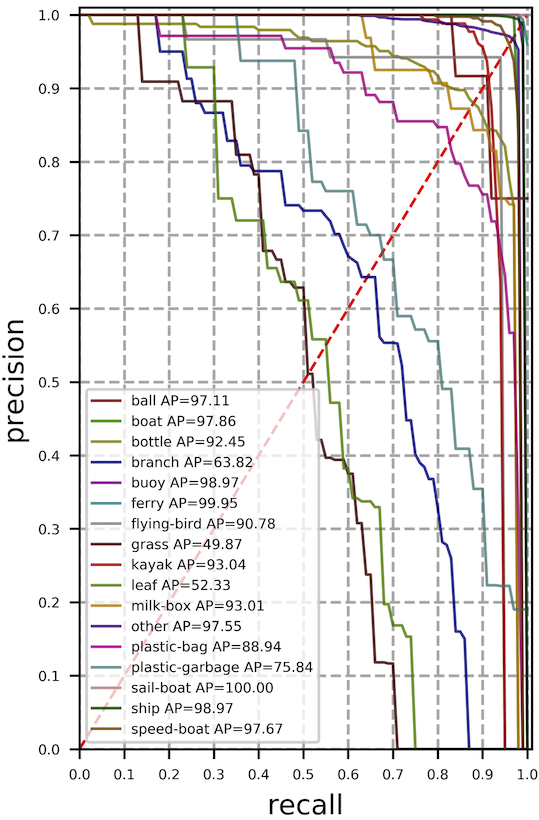
\includegraphics[width=0.46\columnwidth]{images/pr-curve.png}
}
\quad
\subfigure[PRC for PP-YOLO-mobile model (IoU = 0.5)]{
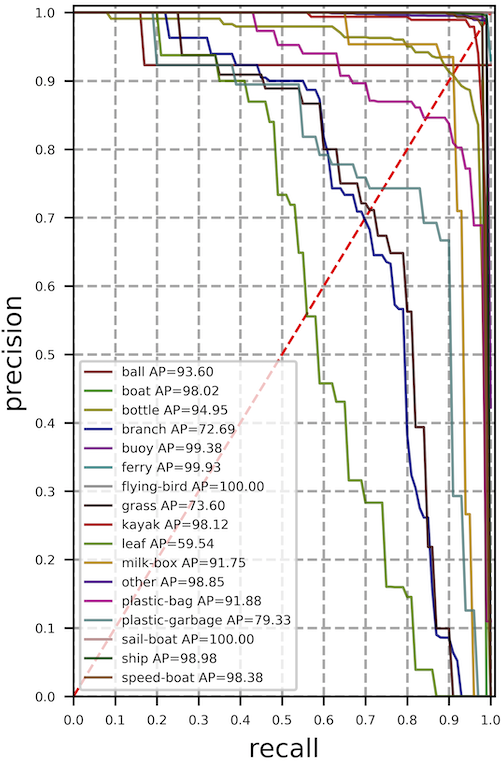
\includegraphics[width=0.46\columnwidth]{images/pr-curve-1.png}
}
\caption{Comparison of ground truth and prediction in the validation set.}
\label{fig:prc}
\end{figure}

It can be seen intuitively from the figure that the PR curve of the PP-YOLO-mobile model is more concentrated in the upper right corner. 
The curve closest to the lower-left corner, that is, the categories with the smallest AP value are grass, leaf, and branch in both figures.
From the point of view of AP value, the grass rises from 49.87 to 72.73, the leaf rises from 52.33 to 59.11, and the branch rises from 63.82 to 67.80. Some other categories, like the bottle, flying-bird, plastic-bag, etc., have a slight increase in AP value from the PP-YOLO-mobile model. This result proves that accuracy can be improved by the PP-YOLO-mobile model.


At this time, a question is raised, why some categories have low AP values, and some have high AP values. Through the classification and analysis of the categories, Table \ref{tbl:Comparison of AP in different dataset} from the original dataset is presented. Categories with high AP value are mostly from the SMD, while the categories with low AP value are from the custom dataset. In the SMD, the target comes from the marine, mainly some fixed-shaped objects which are easy to detect after training. However, the custom dataset contains some objects on the river surface, such as grass, leaves, and branches. They tend to gather together, and their shapes are not fixed, which brings great difficulty to object detection.

\begin{table}[htbp]
\centering
\caption{Comparison of AP in different dataset}
\begin{tabular}{llcc} 
\toprule

\multicolumn{1}{c}{\multirow{2}{*}{\textbf{Dataset}}} &
\multicolumn{1}{c}{\multirow{2}{*}{\textbf{Category}}} &\multicolumn{2}{c}{\textbf{AP}} \\
\cmidrule(l){3-4} 
&& \textbf{PP-YOLO} & \textbf{PP-YOLO-mobile} \\

\midrule
\multirow{7}{*}{Singapore Maritime Dataset} 
& boat& 97.86  & 97.93  \\
& buoy & 98.97 & 98.97 \\
& ferry & 99.95 & 100.00 \\
& flying-bird & 90.78 & 97.10 \\
& kayak & 93.04 & 97.68 \\
& other & 97.55 & 98.69 \\
& sail-boat & 100.00 & 100.00 \\
& ship & 98.97 & 98.97 \\
& speed-boat & 97.67 & 98.33 \\
\cmidrule(r){1-4}

\multirow{8}{*}{Custom Dataset} 
& ball& 97.11  & 93.60 \\
& bottle & 92.45 & 94.31  \\
& branch & 63.82 & 67.80 \\
& grass & 49.87 & 72.73  \\
& leaf & 52.33 & 59.11 \\
& milk-box  & 93.01 & 92.50 \\
& plastic-bag & 88.94 & 92.51 \\
& plastic-garbage & 75.84 & 74.89 \\

\bottomrule
\end{tabular}
\label{tbl:Comparison of AP in different dataset}
\end{table}

\subsubsection{Confusion Matrix}
A confusion matrix is another way of presenting the performance of a classification algorithm. The confusion matrix gives a more intuitive representation of the results and gives a good indication of how well the detection algorithm would work in a real scenario. In this experiment, the goal is to identify different obstacles.

\begin{figure}[htbp]
\centering
\subfigure[Confusion matrix for PP-YOLO model]{
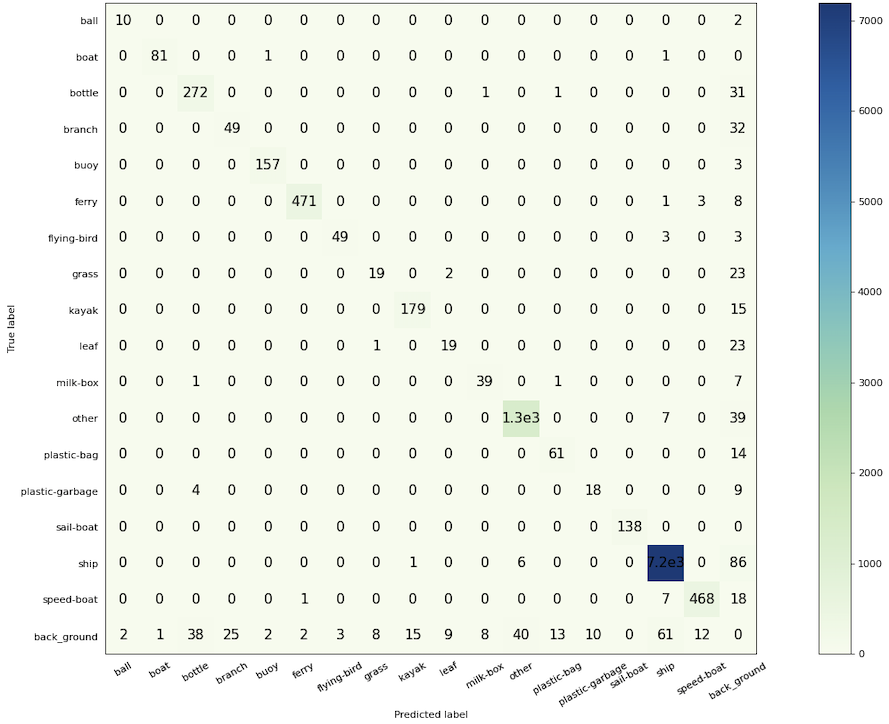
\includegraphics[width=0.9\columnwidth]{images/confusion-matrix.png}
}
\quad
\subfigure[Confusion matrix for PP-YOLO-mobile model]{
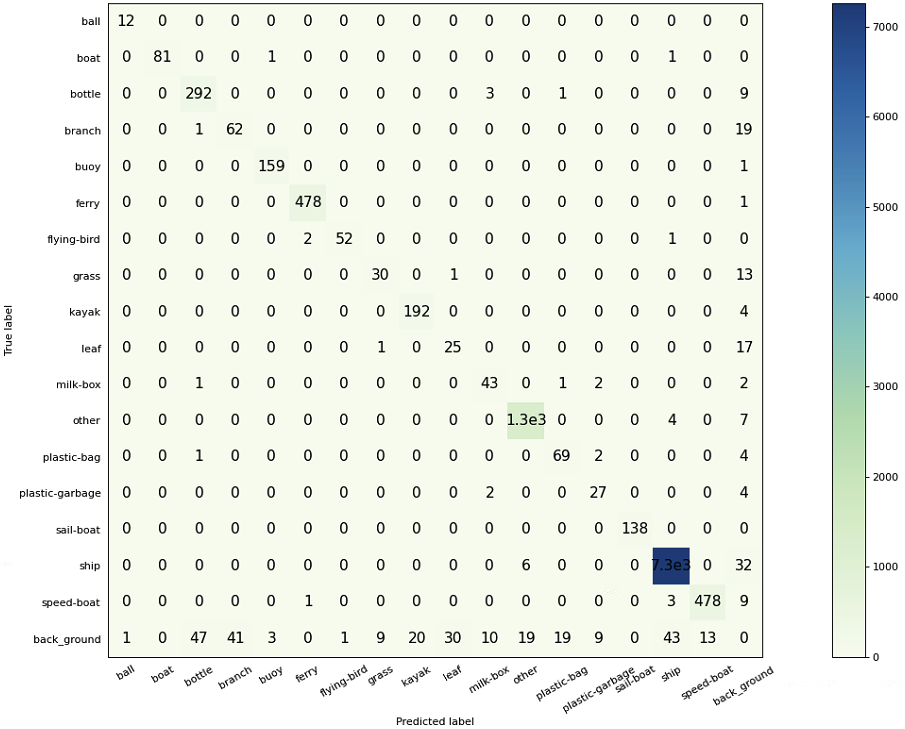
\includegraphics[width=0.9\columnwidth]{images/confusion-matrix-ppyolo-mobile.png}
}
\caption{Comparison of confusion matrix.}
\label{fig:confusion matrix}
\end{figure}

In this section two figures are presented, Figure \ref{fig:confusion matrix} (a) for the PP-YOLO model, and Figure \ref{fig:confusion matrix} (b) for the PP-YOLO-mobile model. In the two figures, the abscissa is the predicted label, and the ordinate is the true label. The value inside shows the relationship between the predicted value and the true value. Most of the values are on the diagonal line, that is, the predicted result is consistent with the real result. However, some of the predicted and true values are not equal, which indicates that they have a similar relationship between them.

For example, in Figure \ref{fig:confusion matrix} (a), four objects that are actually plastic-bag are predicted to bottle, six objects that are actually ship are predicted to other, and seven objects that are actually speed-boat are predicted to ship. In Figure \ref{fig:confusion matrix} (b), the confusion of categories has been improved. Only two objects that are actually plastic-bag are predicted to bottle, five objects that are actually ship are predicted to other, and two objects that are actually speed-boat are predicted to ship. Above all, it can be seen that the PP-YOLO-mobile model reduces the probability of model recognition errors and improves the accuracy of recognition.





\subsubsection{Mean Average Precision}
Average Precision (AP) is the average of the precision value on the PRC. The integral of PRC is used for calculating AP, and the formula is as follows:

\begin{equation} 
{AP} = {\int_{0}^{1}\text{p(r)dr}} 
\end{equation}

Mean Average Precision (mAP) is the average value of AP, that is, the average of the area under the PRC of each category. MAP is an indicator of the overall recognition accuracy in target detection Generally, the higher the mAP value, the better the performance of the model in all categories. The formula is as follows, where $Q$ is the number of categories.

\begin{equation} 
{mAP} = {\frac {\sum _{q=1}^{Q}\operatorname {AP(q)} }{Q}}
\end{equation}

\begin{figure}[htbp]
\centering
\subfigure[mAP for PP-YOLO model]{
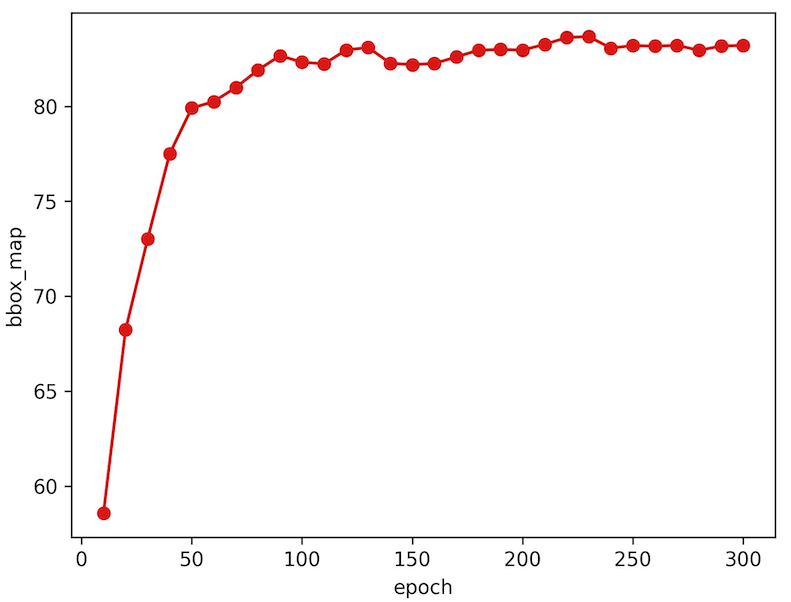
\includegraphics[width=0.45\columnwidth]{images/map-ppyolo.png}
}
\quad
\subfigure[mAP for PP-YOLO-mobile model]{
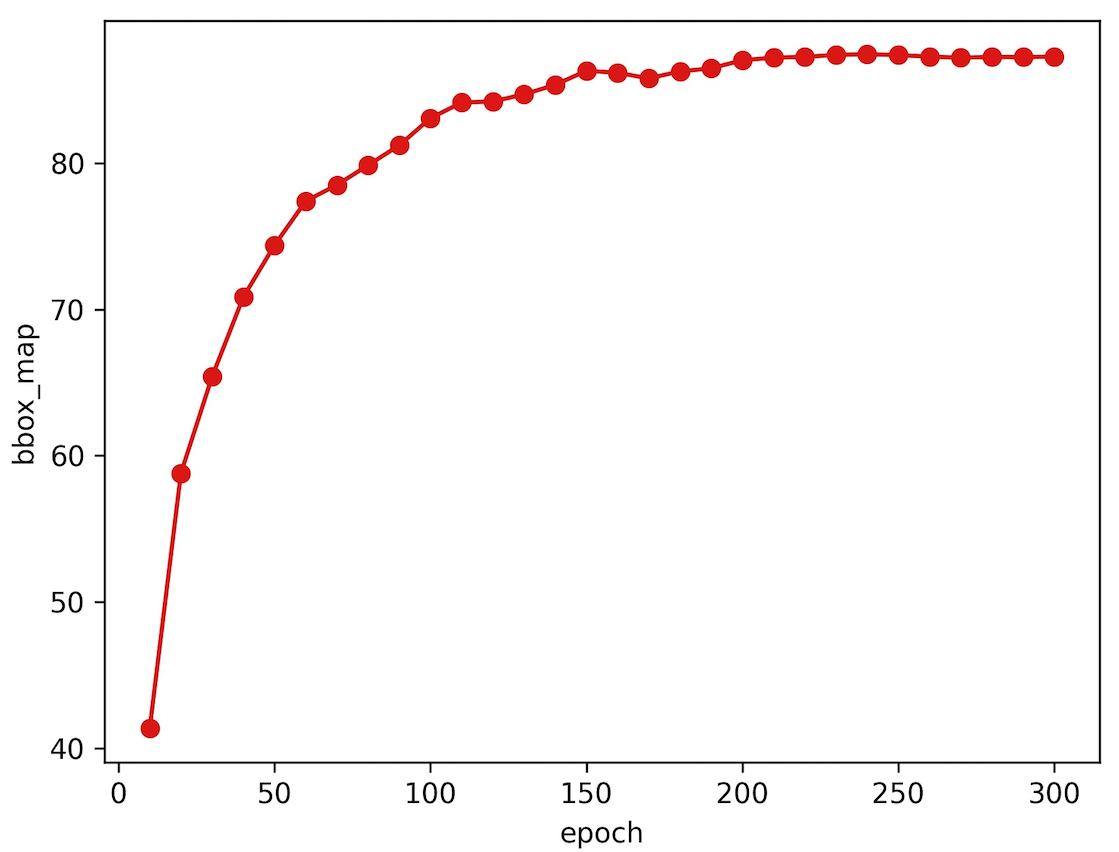
\includegraphics[width=0.45\columnwidth]{images/map-ppyolo-mobile.png}
}
\caption{Comparison of mAP in the validation dataset.}
\label{fig:map}
\end{figure}

As can be seen from Figure \ref{fig:map}, with the increase of epoch, the trend of the mAP of the two models is rising. For the PP-YOLO model, at the 230th epoch, the mAP reached its maximum value of 84.1947. For the PP-YOLO-mobile model, it achieved the best detection result at the 190th epoch, with a value of 86.9339. In the end, the PP-YOLO-mobile model is 2.7392\% higher in accuracy than the PP-YOLO model in this experiment.



From the perspective of the degree of curve rise, the PP-YOLO model has reached 80 in mAP at the 50th epoch, while the PP-YOLO-mobile model needs 90 epochs to achieve this accuracy. This means that complex models have advantages in the number of training epochs, and only a small amount of training is required to achieve relatively high accuracy. After a certain number of training epochs, the mAP values of the PP-YOLO model and the PP-YOLO model both increase slowly or fluctuate slightly, and longer training steps are meaningless.



\subsection{Comparison of Speed}

Frames per second (FPS) is a way to express how fast the method is. It measures the number of images processed on the model per second. The larger the FPS, the faster the model can detect the objects. The calculation formula of FPS is:

\begin{equation} 
{FPS} = \frac {\text{Number\ of\ Images}} {\text{Total\ Seconds}}
\end{equation}

\begin{table}[htbp]
\centering
\caption{Comparison of FPS in the validation dataset}
\begin{tabular}{llll} 
\toprule
\textbf{Model}&\textbf{Total Seconds}&\textbf{Frame Per Second (FPS)}&\textbf{Millisecond Per Frame}\\
\midrule
PP-YOLO model & 47.525&36.822&27\\
PP-YOLO-mobile model&40.058&43.687&23\\
\bottomrule
\end{tabular}
\label{tbl:Comparison of FPS in the validation dataset}
\end{table}

There are 1750 images in the validation set. It takes 47.525 seconds for PP-YOLO model to complete the detection, and 40.058 seconds for the PP-YOLO-mobile model. The value of FPS is usually used to indicate the speed of model detection. Table \ref{tbl:Comparison of FPS in the validation dataset} shows the results of FPS after calculation.

For the PP-YOLO-mobile model, it can detect 43.687 pictures per second, which is 6.865 more pictures than the PP-YOLO model. From another perspective, the PP-YOLO-mobile takes an average of 23 milliseconds per frame, which is four milliseconds less than the PP-YOLO model. In summary, the PP-YOLO-mobile model is faster than the PP-YOLO model in speed for object detection.



\subsection{Ablation Study}

Sine the PP-YOLO-mobile can improve performance by replacing backbone and data enhancement at the same time. However, it is not sure that both of them contribute to the improvement of the model. It is also possible that only one of them can be used to improve performance. Therefore, an ablation study has also been carried out. The results are summarized in Table \ref{tbl:Results of ablation study}, and the histogram for visual comparison is shown in Figure \ref{fig:ablation-bar}.


\begin{table}[htbp]
\centering
\caption{Results of ablation study}
\begin{tabular}{llll} 
\toprule
\textbf{Group}&\textbf{Methods}&\textbf{mAP}&\textbf{FPS}\\
\midrule
A& PP-YOLO + ResNet50 (Benchmark) &84.1947 & 36.822\\
\cmidrule(r){1-4}
B& PP-YOLO + MobileNetV2 &82.7062 & 45.548\\
C& PP-YOLO + ResNet50 + Data Augmentation & 87.5855 & 32.454\\
D& PP-YOLO + MobileNetV2 + Data Augmentation & 86.9339& 43.687\\
\bottomrule
\end{tabular}
\label{tbl:Results of ablation study}
\end{table}

\begin{figure}[htbp]
\centering
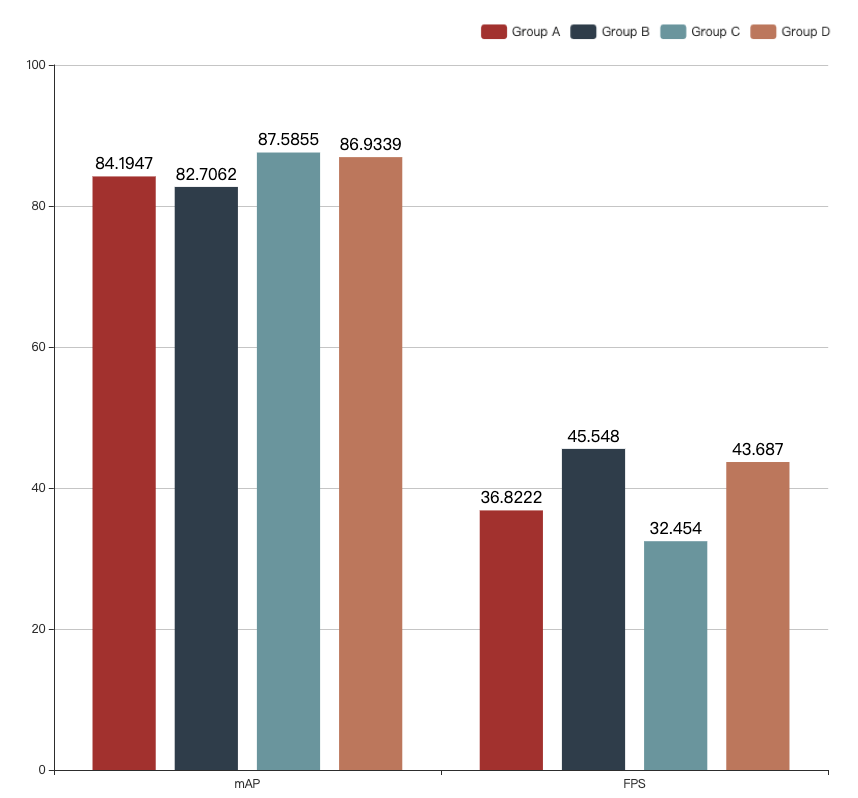
\includegraphics[width=1\columnwidth]{images/ablation-bar.png}
\caption{Histogram of ablation study results.}
\label{fig:ablation-bar}
\end{figure}

Group A and Group D are the PP-YOLO and PP-YOLO-mobile models analyzed previously. Group B is a combination of PP-YOLO algorithm and MobileNetV2 backbone. Compared with the PP-YOLO model, the accuracy has dropped by 1.4885, but the speed has increased by 8.726. Group C has applied data augmentation based on Group A and achieved a precision increase of 3.3908, but FPS also decreased by 4.368.

Above all, Group C has the highest accuracy, and Group B has the fastest speed. Both MobileNetV2 backbone and data augmentation have their own effects, and one of them alone cannot bring about the improvement of overall performance.


\subsection{Performance on Jetson Nano}
Evaluation on the server with Tesla GPU has achieved a good result. In real applications, the performance of the hardware in the developer kit is limited, such as CPU, GPU and memory. Besides, since it is battery powered, the output voltage also affects the performance of the model. Table \ref{tbl:performance on Jetson Nano} shows the results of experiments on Nvidia Jetson Nano.


\begin{table}[htbp]
\centering
\caption{Performance on Jetson Nano}
\begin{tabular}{lllll} 
\toprule
\textbf{Model}&\textbf{Original Size}&\textbf{Size after Pruning}&\textbf{mAP}&\textbf{FPS}\\
\midrule
PP-YOLO  & 219.2MB&33.5MB&83.4048&10.644\\
PP-YOLO-mobile &173.4MB & 26.4MB&86.2752&16.527\\
\bottomrule
\end{tabular}
\label{tbl:performance on Jetson Nano}
\end{table}


After model pruning, the size of the model has been dramatically reduced, from 219.2MB to 33.5MB for the PP-YOLO model and 173.4MB to 26.4MB for the PP-YOLO-mobile model. At the same time, the accuracy of the model is only slightly reduced by 0.7899 and 0.6587. Compared with the PP-YOLO model, PP-YOLO-mobile model has increased by 5.883 in FPS, reaching a value of 16.527.



\subsection{Discussion}
Above all, the performance is compared in a quantitative way for the PP-YOLO-mobile model and the original PP-YOLO model. According to the results, by replacing the ResNet50 backbone with the MobileNetV2 backbone, the speed of model recognition can be improved. Through data augmentation, the accuracy of model recognition can be increased. In detail, the ResNet50 backbone has a larger number of parameters and obviously shows better performance than MobileNetV2. After replacing with the MobileNetV2 backbone, the model becomes simpler, and the detection speed is improved. Furthermore, data augmentation enriches the diversity of training data, and more complex pictures are processed during model training, so that the speed of detection is improved.

In some difficult obstacle recognition, such as in the recognition of leaves, grasses, branches, the accuracy of the PP-YOLO-mobile model recognition has been greatly improved. This means that data enhancement can indeed enrich training samples by adjusting brightness, contrast, cropping, etc., and enhance the ability to handle complex targets. The results of data augmentation are presented in Figure \ref{fig:data agumentation}. 

\begin{figure}[htbp]
\centering
\subfigure[OriginalImage (1920 x 1080 pixels)]{
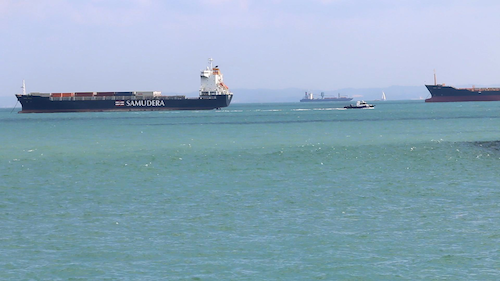
\includegraphics[width=0.4\columnwidth]{images/data-augmentation-1.png}
}
\quad
\subfigure[OriginalImageWithGTBox (1920 x 1080 pixels)]{
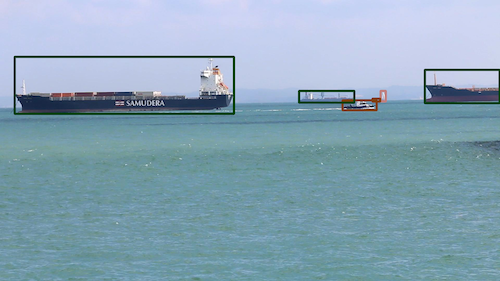
\includegraphics[width=0.4\columnwidth]{images/data-augmentation-2.png}
}
\quad
\subfigure[MixupImage (1920 x 1080 pixels)]{
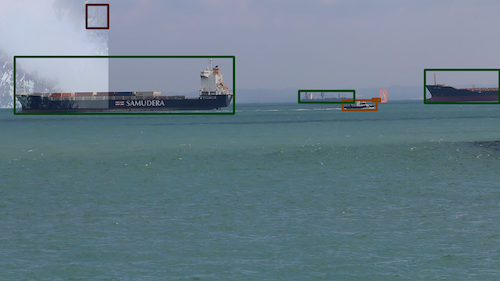
\includegraphics[width=0.4\columnwidth]{images/data-augmentation-3.png}
}
\quad
\subfigure[RandomDistort (1920 x 1080 pixels)]{
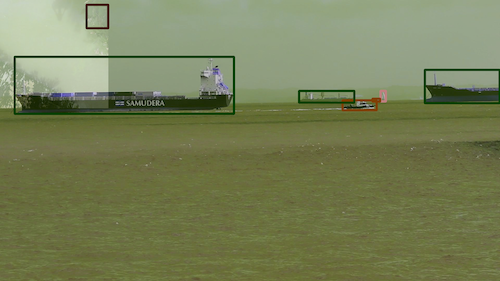
\includegraphics[width=0.4\columnwidth]{images/data-augmentation-4.png}
}
\quad
\subfigure[RandomExpand (4669 x 2626 pixels)]{
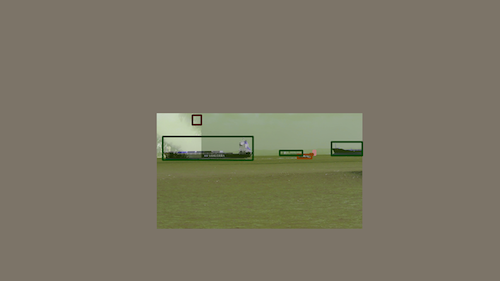
\includegraphics[width=0.4\columnwidth]{images/data-augmentation-5.png}
}
\quad
\subfigure[OriginalCrop (4669 x 2626 pixels)]{
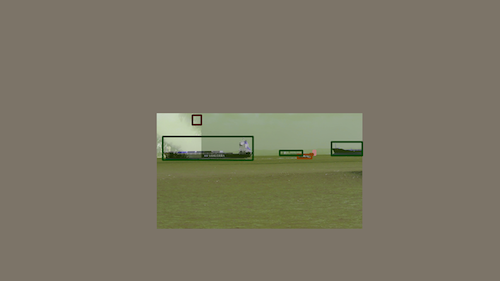
\includegraphics[width=0.4\columnwidth]{images/data-augmentation-6.png}
}
\quad
\subfigure[Resize (608 x 608 pixels)]{
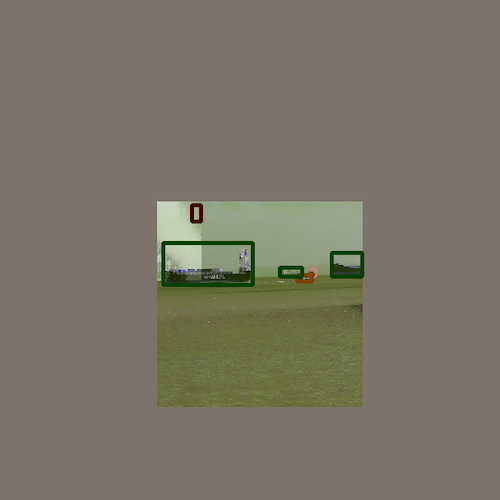
\includegraphics[width=0.24\columnwidth]{images/data-augmentation-7.png}
}
\quad
\subfigure[RandomHorizontalFlip (608 x 608 pixels)]{
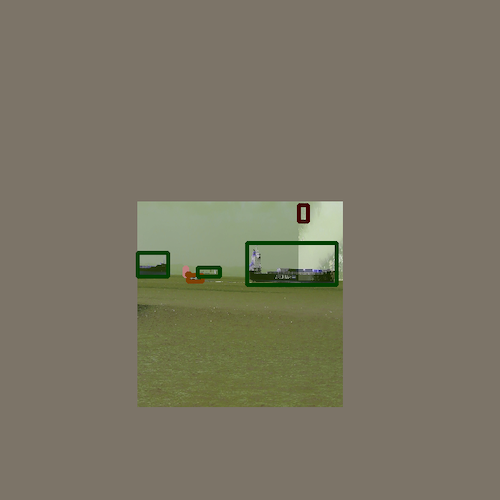
\includegraphics[width=0.24\columnwidth]{images/data-augmentation-8.png}
}
\caption{Sample image after data augmentation. (a) is the original image of 1920 x 1080 pixels. (b) is the original image with ground-truth boxes which indicate obstacles from this image. (c), (d), (e), (f), (g) and (h) demonstrate the image results after each data augmentation method. Finally, images are unified into the size of 608 x 608 pixels.
}
\label{fig:data agumentation}
\end{figure}


To compare the detection effects of the two models vividly, we respectively selected two pictures in the test set from the SMD and custom dataset and drew the visualization pictures under the two models which are displayed in Figure \ref{Comparison of ground truth and prediction for two models in the testing set}. The first row is the pictures with ground-true labels. The second and third lines are their visualization effects under the PP-YOLO model and PP-YOLO-mobile model. 
From the left column, the accuracy of different categories under the PP-YOLO-mobile model has been improved. Accuracy of the ship increased from 0.99 to 1.00, ferry increased from 0.96 to 0.99, and buoy increased from 0.97 to 0.99.
Similarly, the accuracy in the second column has also been improved. The different bottles have been increased from 0.789 to 0.95, 0.75 to 0.90, and 0.94 to 0.96.

\begin{figure}[htbp]
\centering
\subfigure[Ground Truth]{
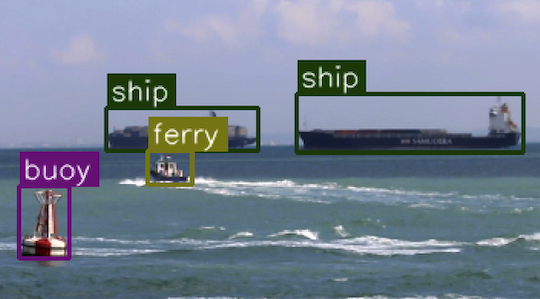
\includegraphics[width=0.47\columnwidth]{images/detection-result-1-1.png}
}
\quad
\subfigure[Ground Truth]{
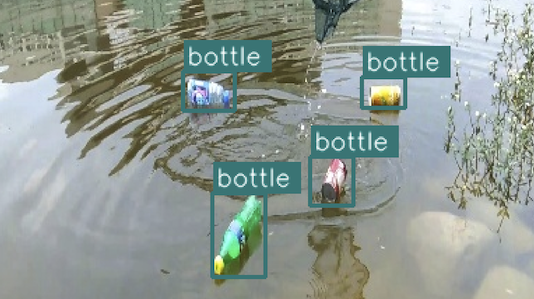
\includegraphics[width=0.47\columnwidth]{images/detection-result-2-1.png}
}
\subfigure[Prediction of the PP-YOLO model]{
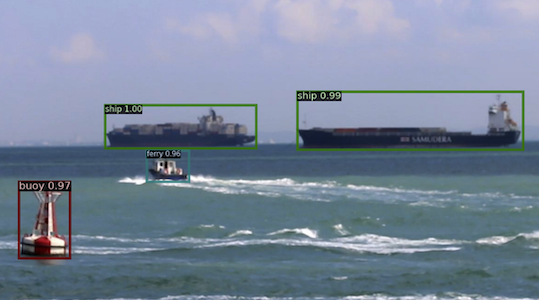
\includegraphics[width=0.47\columnwidth]{images/detection-result-1-2.png}
}
\quad
\subfigure[Prediction of the PP-YOLO model]{
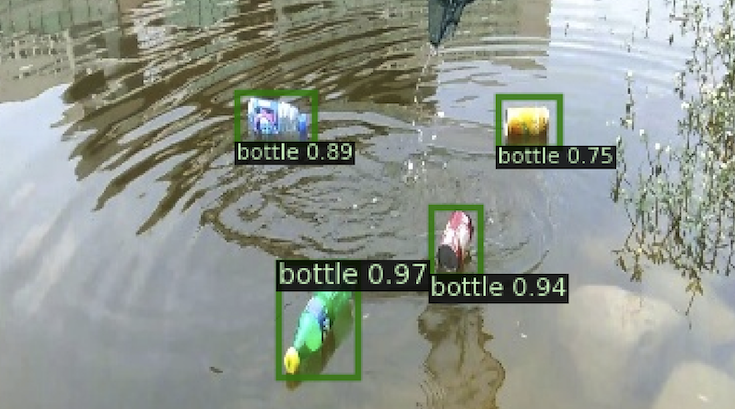
\includegraphics[width=0.47\columnwidth]{images/detection-result-2-2.png}
}

\subfigure[Prediction of the PP-YOLO-mobile model]{
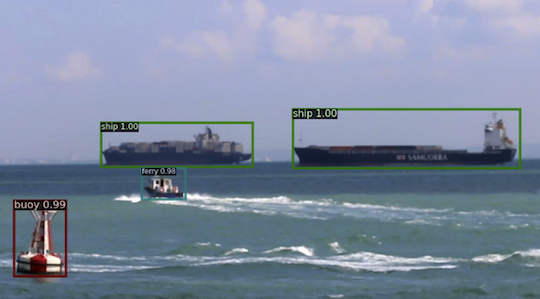
\includegraphics[width=0.47\columnwidth]{images/detection-result-1-3.png}
}
\quad
\subfigure[Prediction of the PP-YOLO-mobile model]{
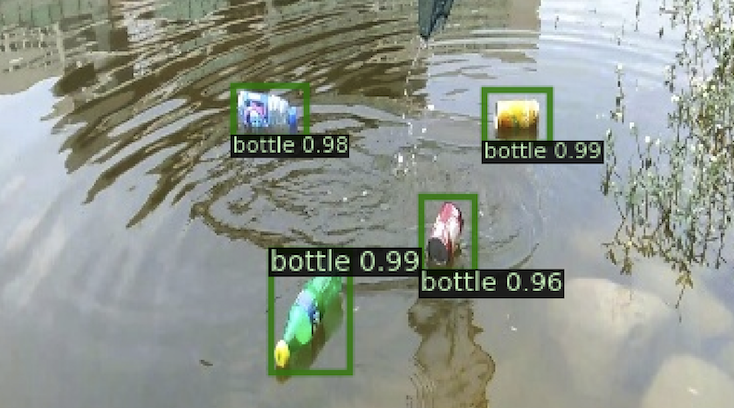
\includegraphics[width=0.47\columnwidth]{images/detection-result-2-3.png}
}
\caption{Comparison of ground truth and prediction for two models in the testing set.}
\label{Comparison of ground truth and prediction for two models in the testing set}
\end{figure}

\section{Conclusion}


As the detection and recognition of obstacles for USVs are challenging, this research aims to construct a model with high accuracy and high speed which can be used in real scenarios. By reading extensive literature and researching on the latest papers, the PP-YOLO algorithm is considered to be the most accurate one-stage algorithm. Compared with the two-stage algorithm, it does not require the region proposal stage and directly generates the class probability and position coordinate value of the object. After a single detection, the final detection result can be directly obtained, so it has a faster detection speed that can be used for USVs.

By replacing the ResNet50 backbone in the original PP-YOLO model with the simpler MobileNetV2 backbone, plus the data augmentation method. The accuracy and speed of the model are improved at the same time. In detail, the accuracy is increased by 2.7392\% in mAP, and the speed is increased by 6.865 in FPS.

By pruning the exported model, the size of the model is reduced from the original 173.4MB to 26.4MB. After being deployed on the Jetson Nano developer kit, the accuracy is 86.2752, and the FPS value is 16.527, which meets the requirements of real-time target detection for USVs.

\subsection{Major Findings}
The results present that the PP-YOLO-mobile model has improved the average accuracy and speed of detection compared with the PP-YOLO model.

\begin{itemize}
\item{The accuracy of the PP-YOLO-mobile model for obstacle detection is 2.7392\% higher than that of the original PP-YOLO model, reaching 86.9339\%.}
\end{itemize}

\begin{itemize}
\item{The processing speed of the PP-YOLO-mobile model is 6.865 faster than that of the PP-YOLO model in FPS, reaching 43.687.}

\end{itemize}

Moreover, through an ablation study, we compared the impact on the model when the backbone replacement and data augmentation are modified separately.
Although the PP-YOLO models with ResNet50 backbone have a larger mAP than the PP-YOLO models with MobileNetV2 backbone, they also have a smaller FPS than other models. The ResNet50 backbone has a complex network structure and many parameters which leads to better performance in mAP and worse performance in FPS.


Our proposed PP-YOLO-mobile belongs to the lightweight deep learning model. They have a relatively simple network structure and few parameters. Although the mAP of our PP-YOLO-mobile model is a reduction compared with the PP-YOLO with data augmentation, the reduction is much smaller than the increase of FPS, and almost can be ignored. According to specific scenarios, our proposed model is more suitable for deploying on embedded devices.


\subsection{Implications}
\subsubsection{Theoretical Implications}
Through this experiment, it is proved that the complex ResNet backbone can improve the accuracy of the model, and the simple MobileNet backbone can increase the speed of the model. From this perspective, it can help researchers choose the appropriate backbone to apply to their models. In addition, the experimental results also show that data augmentation can enrich the number and diversity of the dataset so that the accuracy of the model can be improved after training. The findings of this study have constructive significance for the improvement of model accuracy in future studies.

\subsubsection{Practical Implications}
In terms of practical application, this research has realised the detection of obstacles on the water surface based on computer vision. Compared with other sensors, it can clearly perceive the appearance of obstacles, so as to realise the category recognition of obstacles.
Some of these categories may not be called obstacles, but they can be used as statistics of river pollution after identifying, which is also very helpful for pollutant detection and environmental monitoring. 
Besides, this experiment provides a lightweight object detection model that can not only be applied to USVs but also can be migrated to other applications that use embedded devices, such as UAVs and robots.


\subsection{Contributions}
Through the whole process of the experiment, this research has achieved the following contributions:

\begin{enumerate}

\item Create a dataset of obstacles on the water surface, containing 17 categories, 8750 pictures with all label information.
\item Propose a PP-YOLO-mobile model which has improved the original PP-YOLO model in accuracy and speed by backbone replacement and data augmentation.
\item Generate an inference model with a size of only 26.4MB, with mAP of 86.2752 and FPS of 16.527 on the USV dataset.

\end{enumerate}

\subsection{Limitations}
Although every effort has been made to eliminate design and analysis flaws, there are inevitably some limitations, which should be considered when conducting further research.

So far, there are few public datasets of floating objects on the Internet. Categories of water obstacle data collected in this experiment are also limited. Although some data augmentation methods are used in the model to expand the dataset, it is still impossible to cover all obstacle categories. The USV needs to sail more times and collect more data in areas with more complex environments. Not only the number of images need to be expanded, but the diversity of data need to be increased.

Besides, from experiments in real scenes, we found that in the case of high winds, water splashes are sometimes mistaken for obstacles such as birds, which affect the normal navigation for the USVs. In addition, the shaking of the camera on the water and the water splashing on the lens will also affect the recognition of obstacles. Therefore, a camera with anti-shake and lens heating function is essential.

Finally, obstacles under the water also need to be considered in the next research. For example, there may be some obstacles that have a small part on the water surface but a larger part under the water, which will cause misjudge and collision. Sensors such as sonar need to be fused to the USVs to form a coordinated detection of obstacles on the water surface and underwater.


\subsection{Further Study}

All these limitations may affect the performance of obstacle detection and recognition for USVs. Thus, future research designs will take individual factors into consideration. In terms of models, we will continue to study the latest and best target detection algorithms and some improvement skills. Usually, those optimal algorithms are generated on servers with better performance, some improvements need to be done on the models to meet the requirements of the embedded developer kit.

After the obstacle is detected, the distance between the USV and the obstacle also needs to be measured. The camera has disadvantages in measuring distance in which the accuracy of distance measurement is easily affected by the environment. The millimeter-wave radar has a strong ability to resist environmental interference and can meet the requirements of adaptability to the all-weather climate. Therefore, an essential task we plan to carry out in the next step is to combine the advantages of radar and camera to detect and recognize obstacles.



%%%%%%%%%%%%%%%%%%%%%%%%%%%%%%%%%%%%%%%%%%

\vspace{6pt} 

\funding{This work was partly supported by the AI University Research Centre (AI-URC) through XJTLU Key Programme Special Fund (KSF-P-02 and KSF-A-19) and Research Development Fund of XJTLU (RDF-19-02-23).}

\conflictsofinterest{The authors declare no conflict of interest.} 


%%%%%%%%%%%%%%%%%%%%%%%%%%%%%%%%%%%%%%%%%%

%%%%%%%%%%%%%%%%%%%%%%%%%%%%%%%%%%%%%%%%%%
\end{paracol}
\reftitle{References}

% Please provide either the correct journal abbreviation (e.g. according to the “List of Title Word Abbreviations” http://www.issn.org/services/online-services/access-to-the-ltwa/) or the full name of the journal.
% Citations and References in Supplementary files are permitted provided that they also appear in the reference list here. 

%=====================================
% References, variant A: external bibliography
%=====================================
\externalbibliography{yes}
\bibliography{reference.bib}



% If authors have biography, please use the format below
%\section*{Short Biography of Authors}
%\bio
%{\raisebox{-0.35cm}{\includegraphics[width=3.5cm,height=5.3cm,clip,keepaspectratio]{Definitions/author1.pdf}}}
%{\textbf{Firstname Lastname} Biography of first author}
%
%\bio
%{\raisebox{-0.35cm}{\includegraphics[width=3.5cm,height=5.3cm,clip,keepaspectratio]{Definitions/author2.jpg}}}
%{\textbf{Firstname Lastname} Biography of second author}

% The following MDPI journals use author-date citation: Arts, Econometrics, Economies, Genealogy, Humanities, IJFS, JRFM, Laws, Religions, Risks, Social Sciences. For those journals, please follow the formatting guidelines on http://www.mdpi.com/authors/references
% To cite two works by the same author: \citeauthor{ref-journal-1a} (\citeyear{ref-journal-1a}, \citeyear{ref-journal-1b}). This produces: Whittaker (1967, 1975)
% To cite two works by the same author with specific pages: \citeauthor{ref-journal-3a} (\citeyear{ref-journal-3a}, p. 328; \citeyear{ref-journal-3b}, p.475). This produces: Wong (1999, p. 328; 2000, p. 475)

%%%%%%%%%%%%%%%%%%%%%%%%%%%%%%%%%%%%%%%%%%
%% for journal Sci
%\reviewreports{\\
%Reviewer 1 comments and authors’ response\\
%Reviewer 2 comments and authors’ response\\
%Reviewer 3 comments and authors’ response
%}
%%%%%%%%%%%%%%%%%%%%%%%%%%%%%%%%%%%%%%%%%%
\end{document}

